%%%%%%%%%%%%%%%%%%%%%%%%%%%%%%%%%%%%%%%%%%%%%%%%%%%%%%%%%%%%%%%%%%%%%%%%%%%%%%%
%                       CARREGA DE LA CLASSE DE DOCUMENT                      %
%                                                                             %
% Les opcions admissibles son:                                                %
%      12pt / 11pt            (cos dels tipus de lletra; no feu servir 10pt)  %
%                                                                             %
% catalan/spanish/english     (llengua principal del treball)                 %
%                                                                             % 
% french/italian/german...    (si necessiteu fer servir alguna altra llengua) %
%                                                                             %
% listoffigures               (El document inclou un Index de figures)        %
% listoftables                (El document inclou un Index de taules)         %
% listofquadres               (El document inclou un Index de quadres)        %
% listofalgorithms            (El document inclou un Index d'algorismes)      %
%                                                                             %
%%%%%%%%%%%%%%%%%%%%%%%%%%%%%%%%%%%%%%%%%%%%%%%%%%%%%%%%%%%%%%%%%%%%%%%%%%%%%%%

\documentclass[12pt,spanish,listoffigures,listoftables]{tfgetsinf}

%%%%%%%%%%%%%%%%%%%%%%%%%%%%%%%%%%%%%%%%%%%%%%%%%%%%%%%%%%%%%%%%%%%%%%%%%%%%%%%
%                     CODIFICACIO DEL FITXER FONT                             %
%                                                                             %
%    windows fa servir normalment 'ansinew'                                   %
%    amb linux es possible que siga 'latin1' o 'latin9'                       %
%    Pero el mes recomanable es fer servir utf8 (unicode 8)                   %
%                                          (si el vostre editor ho permet)    % 
%%%%%%%%%%%%%%%%%%%%%%%%%%%%%%%%%%%%%%%%%%%%%%%%%%%%%%%%%%%%%%%%%%%%%%%%%%%%%%%

\usepackage[utf8]{inputenc} 

%%%%%%%%%%%%%%%%%%%%%%%%%%%%%%%%%%%%%%%%%%%%%%%%%%%%%%%%%%%%%%%%%%%%%%%%%%%%%%%
%                        ALTRES PAQUETS I DEFINICIONS                         %
%                                                                             %
% Carregueu aci els paquets que necessiteu i declareu les comandes i entorns  %
%                                          (aquesta seccio pot ser buida)     %
%%%%%%%%%%%%%%%%%%%%%%%%%%%%%%%%%%%%%%%%%%%%%%%%%%%%%%%%%%%%%%%%%%%%%%%%%%%%%%%



%%%%%%%%%%%%%%%%%%%%%%%%%%%%%%%%%%%%%%%%%%%%%%%%%%%%%%%%%%%%%%%%%%%%%%%%%%%%%%%
%                        DADES DEL TREBALL                                    %
%                                                                             %
% titol, alumne, tutor i curs academic                                        %
%%%%%%%%%%%%%%%%%%%%%%%%%%%%%%%%%%%%%%%%%%%%%%%%%%%%%%%%%%%%%%%%%%%%%%%%%%%%%%%

\title{Interconexión del robot NAO a servicios de simulación en la nube}
\author{Carmona Vila, Jahel}
\tutor{Blanes Noguera, Juan Francisco}
\curs{2018-2019}

%%%%%%%%%%%%%%%%%%%%%%%%%%%%%%%%%%%%%%%%%%%%%%%%%%%%%%%%%%%%%%%%%%%%%%%%%%%%%%%
%                     PARAULES CLAU/PALABRAS CLAVE/KEY WORDS                  %
%                                                                             %
% Independentment de la llengua del treball, s'hi han d'incloure              %
% les paraules clau i el resum en els tres idiomes                            %
%%%%%%%%%%%%%%%%%%%%%%%%%%%%%%%%%%%%%%%%%%%%%%%%%%%%%%%%%%%%%%%%%%%%%%%%%%%%%%%

\keywords{NAO, simulador, diabetes, HTTP, MQTT} % Paraules clau 
         {NAO, simulador, diabetes, HTTP, MQTT} % Palabras clave
         {NAO, simulator, diabetes, HTTP, MQTT}        % Key words

%%%%%%%%%%%%%%%%%%%%%%%%%%%%%%%%%%%%%%%%%%%%%%%%%%%%%%%%%%%%%%%%%%%%%%%%%%%%%%%
%                              INICI DEL DOCUMENT                             %
%%%%%%%%%%%%%%%%%%%%%%%%%%%%%%%%%%%%%%%%%%%%%%%%%%%%%%%%%%%%%%%%%%%%%%%%%%%%%%%

\begin{document}

\begin{abstract}
En aquest projecte es desenvolupen serveis en el núvol per tal de desacoblar de dins del robot NAO el codi que executa el simulador de diabetes que duu implementat. Es suprimeixen les connexions TCP per protocols de capes superiors en la pila TCP/IP com son HTTP i MQTT que permeten una comunicació més flexible i amb més opcions. A més, es modernitza el codi de manera que sigue més senzilla tant la seva estructura com la seva compilació i execució.
\end{abstract}
\begin{abstract}[spanish]
En este proyecto se desarrollan servicios en la nube para desacoplar de dentro del robot NAO el código que ejecuta el simulador de diabetes que lleva implementado. Se suprimen las conexiones TCP por protocolos de capas superiores en la pila TCP/IP como son HTTP y MQTT que permiten una comunicación más flexible y con más opciones. Además, se moderniza el código para que sea más sencilla tanto su estructura como su compilación y ejecución.
\end{abstract}
\begin{abstract}[english]
In this project are developed cloud services to disengage the code inside the NAO Robot that starts up the diabetes simulator. TCP connectios are suppressed by higher layer protocols in the TCP/IP stack as HTTP and MQTT are which allow a more flexible communication and with more options. Besides the code is modernized so that this can be simplier in terms of structure, compilation and execution.
\end{abstract}

%%%%%%%%%%%%%%%%%%%%%%%%%%%%%%%%%%%%%%%%%%%%%%%%%%%%%%%%%%%%%%%%%%%%%%%%%%%%%%%
%                              CONTINGUT DEL TREBALL                          %
%%%%%%%%%%%%%%%%%%%%%%%%%%%%%%%%%%%%%%%%%%%%%%%%%%%%%%%%%%%%%%%%%%%%%%%%%%%%%%%

\mainmatter

%%%%%%%%%%%%%%%%%%%%%%%%%%%%%%%%%%%%%%%%%%%%%%%%%%%%%%%%%%%%%%%%%%%%%%%%%%%%%%%
%                                  INTRODUCCIO                                %
%%%%%%%%%%%%%%%%%%%%%%%%%%%%%%%%%%%%%%%%%%%%%%%%%%%%%%%%%%%%%%%%%%%%%%%%%%%%%%%

\chapter{Introducción}

\section{Motivación}

Este proyecto desarrollado parte directamente de <<\textit{Desarrollo de un sistema de monitorización y control de un robot simulador de diabetes}>>, un trabajo anterior a éste, el cual se encuentra en Riunet \cite{TFMAnterior}, elaborado por Antonio Bengochea Carrasco y dirigido también por Francisco José Blanes Noguera. Lo que se trata en el actual proyecto es de mejorar la infraestructura anterior teniendo en cuenta las limitaciones sobre las prestaciones que existen hoy en día para el proyecto previo. El centro del proyecto se encuentra dentro del robot NAO, por lo que es el que limita el crecimiento de la aplicación. \\

NAO es un robot humanoide programable y autónomo, desarrollado por Aldebaran Robotics, una empresa francesa con sede en París subsidiaria del grupo Softbank. Estos robots son ampliamente utilizados en por ejemplo la Robocup, un concurso de robótica a nivel internacional. \\

\begin{figure}[!h]
	\centering
	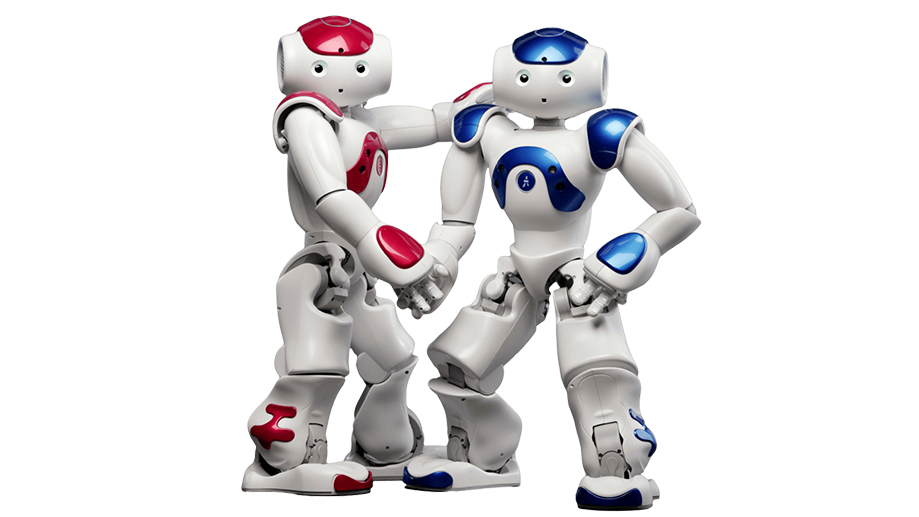
\includegraphics[height=5.5cm]{img/NAOIlustracion}
	\caption{Robot NAO en varios colores}
	\label{figura:NAOIlustracion}
\end{figure}

En esta hoja técnica \cite{NAOdatasheet} se detallan las características técnicas del robot que es objeto de estudio. Con unas dimensiones de 574x275x311mm y un peso de 5.4 kg, el robot consigue su movilidad mediante motores de corriente continua sin escobillas, siendo un total de 26 motores. En la imagen \ref{figura:NAOCinematica} podemos ver su esquema cinemático, en el cual se ven los ángulos de rotación y traslaciones. \\

\begin{figure}[!h]
	\centering
	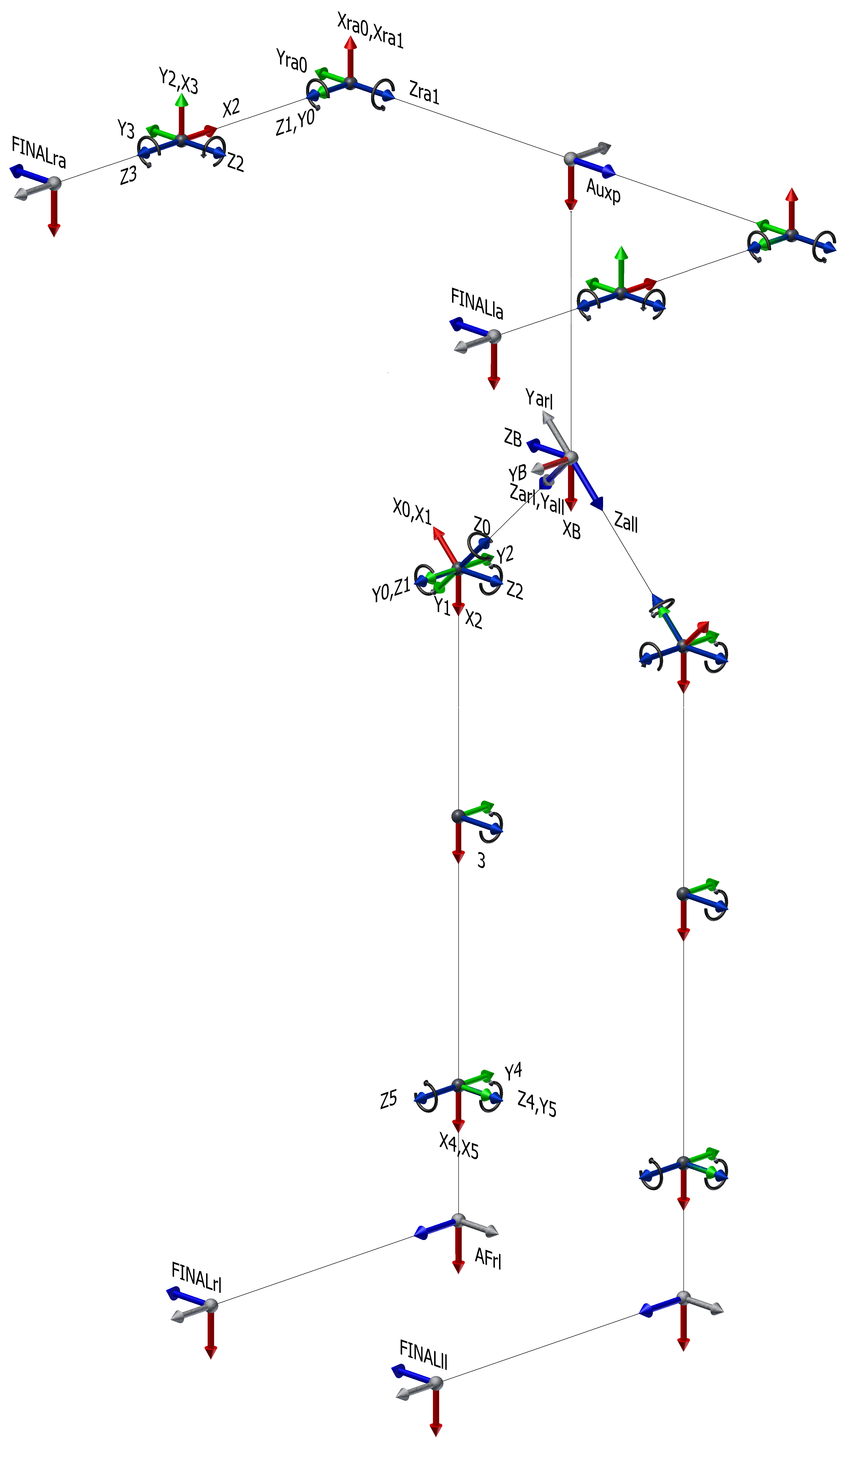
\includegraphics[height=10cm]{img/NAOCinematico}
	\caption{Esquema cinemático del robot NAO.}
	\label{figura:NAOCinematica}
\end{figure}

Como se ha mencionado antes, este proyecto parte de un proyecto anterior, cuyas limitaciones del propio robot suponen a su vez límites en el crecimiento de los procesos que lleva implementados. Precisamente, el componente que ejerce de tope es la unidad de cómputo y sus elementos asociados, como las memorias, o lo que el fabricante denomina \textit{Motherboard}. El límite es debido a que el robot incluye un simulador de diabetes que emplean librerías científicas. Esto supone un uso exhaustivo de los recursos de cómputo del robot, siendo que además del propio simulador, también corren otros procesos e hilos. Las características del robot para este aspecto podemos verlas en la tabla \ref{tabla:motherboardnao}: \\

\begin{table}[h]
\begin{center}
\begin{tabular}{|l|l|r|}
	\hline 
	\textbf{Elemento} & \textbf{Subelemento} & \textbf{Prestaciones} \\ 
	\hline 
	\textbf{CPU} & CPU Processor & Intel ATOM Z530 \\ 
	\hline 
	& Cache memory  & 512KB \\ 
	\hline 
	& Clock speed & 1.6GHz \\ 
	\hline 
	& FSB speed & 533MHz \\ 
	\hline 
	\textbf{RAM} &  & 1GB \\ 
	\hline 
	\textbf{Flash memory} &  & 2GB \\ 
	\hline 
	\textbf{Micro SDHC} &  & 8GB \\ 
	\hline 
\end{tabular} 
\caption{Motherboard del robot NAO}
\label{tabla:motherboardnao}
\end{center}
\end{table}

Para las aplicaciones de hoy en día, 1GB en memoria principal (RAM) es demasiado poco. Además teniendo en cuenta que aparte de ejecutar el código, que es muy cargante como se ha mencionado, también ejecuta otros procesos como por ejemplo la comunicación con sus actuadores y sensores mediante \textit{proxyes} como denomina el fabricante, o por ejemplo la comunicación via HTTP, SSH, entre otros. Por otra parte, el procesador Intel ATOM tienen un rendimiento bajo, como se muestra en a figura \ref{figura:IntelAtom}. No aparece el modelo de NAO, Atom Z530, pero el rendimiento es similar a los modelos que se muestran en la imagen. \\

\begin{figure}[!h]
	\centering
	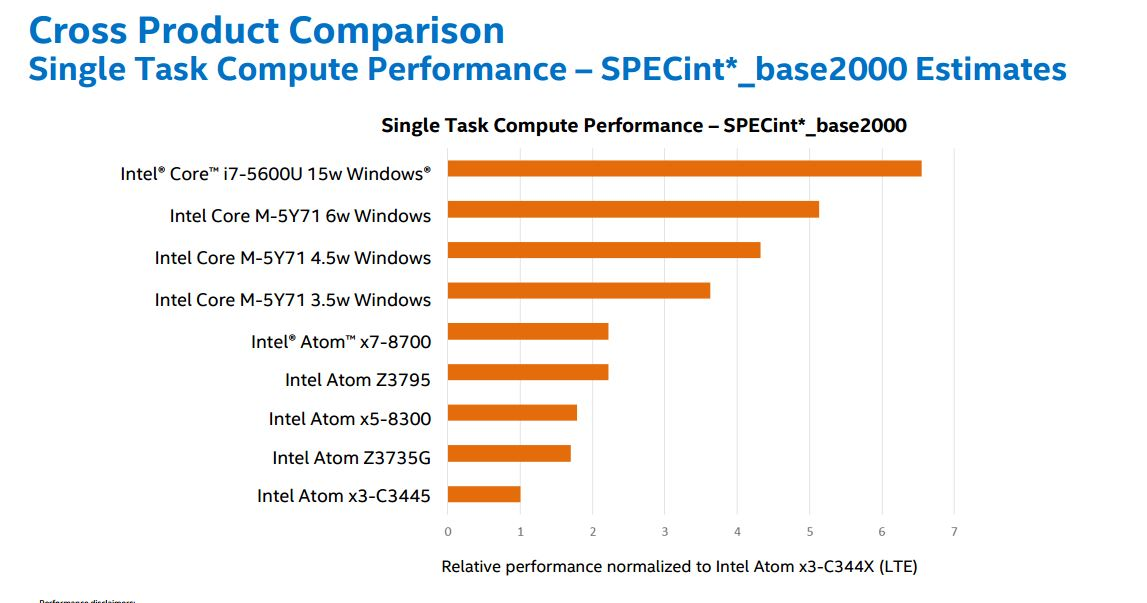
\includegraphics[height=7cm]{img/IntelAtom}
	\caption{Comparativa de rendimiento de procesadores Intel.}
	\label{figura:IntelAtom}
\end{figure}

Es importante entender que el modelo de comportamiento del páncreas que se sigue para simular la diabetes es el modelo \textbf{Hovorka}, cuya implementación puede encontrarse en sus documentos de investigación publicados, como por ejemplo \textbf{TODO: CITAR BIEN EL MODELO DE PANCREAS}. Su resolución pasa por ecuaciones diferenciales que se ejecutan periódicamente, lo cual resulta muy pesado para una máquina de las características que se han observado.

\section{Repaso del proyecto anterior}

El proyecto anterior estaba dividido en dos partes. La primera parte es la que actúa de \textbf{parte servidora} y se encuentra en el código del robot NAO. Mediante conexiones TCP, atiende peticiones de un cliente Java para obtener datos de la glucosa o para recibir órdenes. Contiene dentro cuatro hilos de ejecución, siendo el primero el hilo principal, que incluye un gestionador de hilos; el segundo el hilo que atiende las conexiones TCP; el tercero aloja el código del simulador, y por último, hay dos hilos excluyentes, es decir, que solamente puede haber uno activo cada vez. Estos son un hilo de escenario, que ejecuta el comportamiento de una persona con diabetes, atendiendo al estado de glucosa que tiene en un mismo instante y con funciones de inyectarse insulina. El otro hilo es un hilo de interacción, en el que solamente recibe órdenes sencillas y responde a ellas. \\

La otra parte del proyecto anterior es un \textbf{cliente Java}, el cual en el presente proyecto se va a dejar prácticamente intacto, pues solo va a sustituirse la parte del cliente TCP. Por lo demás, la interfaz solicita al servidor datos de glucosa actual al simulador de diabetes y envía órdenes al robot, que pueden ser acciones sobre los hilos o bien órdenes para que el robot ejecute movimientos o diga palabras.

\section{Objetivo}

El objetivo de este proyecto es \textbf{desengarzar la parte pesada del código del anterior proyecto para virtualizarla en un servicio en la nube}. Esta parte es el simulador de diabetes, que implementa ecuaciones muy costosas computacionalmente y emplea librerías científicas. \\

Esto implica una transformación total de la parte del código de NAO, que significa actualizar las partes del proyecto <<\textit{Desarrollo de un sistema de monitorización y control de un robot simulador de diabetes}>>. Se ha eliminado completamente TCP de la estructura del proyecto y se ha sustituido por MQTT o HTTP (REST), según necesidad. Las partes del proyecto por lo tanto necesitan estas modificaciones: 
\begin{itemize}
	\item Aplicación Java: En vez de utilizar una conexión TCP para conectarse al robot, deberá utilizar librerías para hacer llamadas HTTP y un cliente MQTT. 
	\item La parte de NAO: Sufre un cambio radical ya que se debe cambiar de C++ a Python 2.7 como se justifica en la sección \ref{CambioPython}, y se divide el proyecto en dos partes:
		\subitem -- Google Cloud Engine: Se debe alquilar un servicio en la nube, en este caso del proveedor Google, y se montará un servidor que atenderá peticiones HTTP. Las responderá con el estado de la glucosa actualmente, ya que contendrá el simulador de diabetes.
		\subitem -- Código en NAO: Se debe eliminar toda la parte del simulador y TCP. Se añadirán dos librerías de HTTP y un cliente MQTT. 
\end{itemize}

\section{Estructura de la memoria}

Este proyecto se va a dividir en cuatro partes, que corresponden a las tres partes que conforman el proyecto y una cuarta sobre cómo se relacionan entre ellas. Las tres partes son las mencionadas en la sección anterior: Cliente Java, servicio en la nube y código en NAO. \\

Finalmente, se valorará el resultado del proyecto mediante unas conclusiones y se listarán una serie de posibles mejoras al proyecto actual. También hay un apéndice con información técnica acerca de cómo configurar los diferentes servicios.

\newpage
\chapter{Servicio en la nube}

\section{Servicios en la nube actualmente}

Hoy en día existen empresas que ofrecen lo que se llama \textit{Cloud computing}, o lo que es lo mismo, computación en la nube o servicios en la nube, es un paradigma que permite ofrecer servicios de computación a través de una red, que usualmente es Internet. \\

La computación en la nube físicamente son servidores encargados de atender las peticiones recibidas en cualquier momento. Sirven a sus usuarios desde varios proveedores de alojamiento repartidos por todo el mundo. Este comportamiento está esquematizado en la figura \ref{figura:cloudcomputescheme}. Esta medida reduce los costos, garantiza un mejor tiempo de actividad y que los sitios web sean mucho más seguros. \\

\begin{figure}[!h]
	\centering
	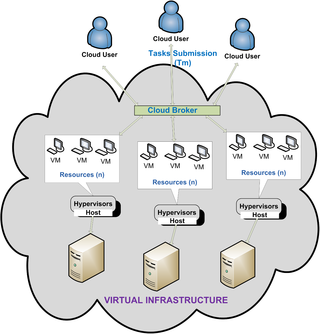
\includegraphics[height=7cm]{img/cloudcompute}
	\caption{Esquema de servicios en la nube.}
	\label{figura:cloudcomputescheme}
\end{figure}

Los servicios en la nube pueden ofrecer cierto nivel de servicios. Esto permite que, si se ofrece un nivel alto de servicio, el programador se ahorra tener que desarrollar la aplicación, pero la parte personalizable queda reducida. Por contra, si se contrata un nivel de servicio bajo, el programador deberá invertir tiempo en desarrollar la aplicación sobre el servicio y será mucho más personalizable. Estos tipos de nivel de servicio son:

\begin{itemize}
	\item \textbf{Iaas (Infraestructure as a Service)}: Permite gestionar al desarrollador aspectos como el sistema operativo, qué servidores quiere instalar en su máquina... Pero los aspectos hardware se hacen transparentes al programador. Un ejemplo de esto es el Google Compute Engine, ya que permite crear máquinas virtuales en las que se puede ejecutar cualquier tipo de software dentro.
	\item \textbf{Paas (Platform as a Service)}: Está un nivel por encima de IaaS, porque se hacen transparentes al programador, además de lo anterior, aspectos de sistema operativo, servicios de una máquina virtual... De manera que el desarrollador solamente debe rellenar algunas secciones de código. Un ejemplo de PaaS sería Google App Engine, ya que es una plataforma que permite redireccionar mediante peticiones REST aquellas peticiones a los fragmentos de código que ha escrito el programador.
	\item \textbf{Saas (Software as a Service)}: Cualquier servicio en la web listo para ser usado tal como está. Estos son los que los usuarios conocen más, porque son por ejemplo Google Drive, entre otros.
\end{itemize}

\begin{figure}[!h]
	\centering
	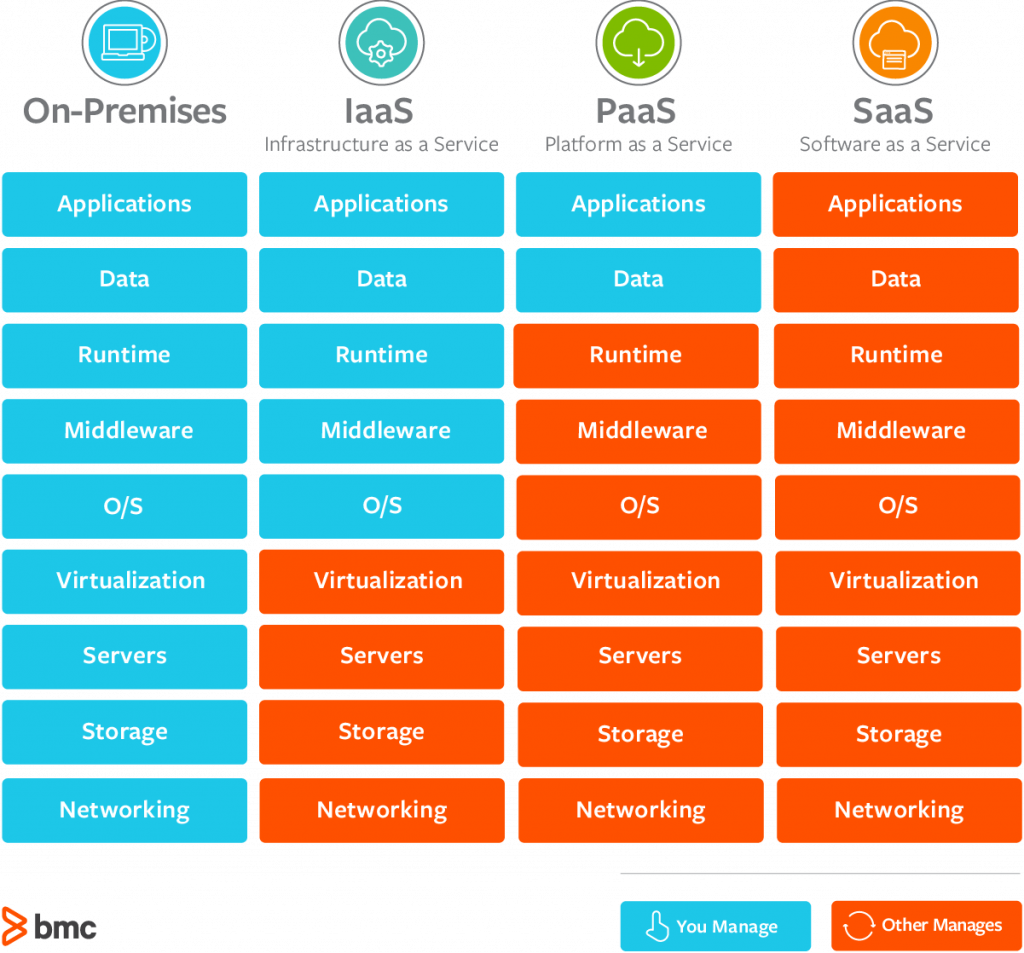
\includegraphics[height=7cm]{img/iaas_saas_paas}
	\caption{Niveles de servicio: IaaS, SaaS y PaaS.}
	\label{figura:IaasSaasPaas}
\end{figure}

En la figura \ref{figura:IaasSaasPaas} se aprecian las distintas capas que cubre cada uno de los niveles de servicio. Aparece uno no nombrado hasta ahora que es \textit{On-premises}; básicamente, se refiere a cómo serían los servicios localmente. \\

Hoy en día los mayores proveedores de servicios en la nube que existen son Amazon Web Services, IBM, Oracle, Alibaba, Google Cloud Services y Microsoft Azure. De las compañías mencionadas, las más grande y empleada en el mundo empresarial es Amazon Web Services, pero en este proyecto no se ha seleccionado debido a que la complejidad de su nube es muy alta, ya que ofrecen un total de 2400 aplicaciones como se indica en esta tabla \cite{ComparativaCloud}. Se ha escogido una más sencilla como es \textbf{Google Cloud Services}, que ocupa el tercer lugar y con una curva de aprendizaje mucho más rápida que sus anteriores. Además, el plan económico de Google Cloud Services es mucho más conveniente que otros. \\

\section{Google Cloud Services}

De la gama que ofrece Google Cloud Services, de la cual podemos ver una muestra en la imagen \ref{figura:googlecloudproducts} se han estado contemplando varias opciones. En un primer lugar, se estuvo barajando trabajar con Google App Engine, que como se ha nombrado antes, es un PaaS. Así, el trabajo a realizar se consideraría notablemente. Pero tuvo que descartarse debido a que ciertas partes como la concurrencia de hilos no eran compatibles con el diseño del PaaS. Se estuvieron mirando otros productos para complementarlo, como son Google Tasks o Google Cloud Storage, pero la combinación no podían generar un servicio de simulación de diabetes en la nube, como era el propósito. Para tener más libertad, se ha escogido para este proyecto un \textbf{IaaS}, \textbf{Google Compute Engine}, porque tiene mucha flexibilidad para programar los servicios que se deseen. \\

\begin{figure}[!h]
	\centering
	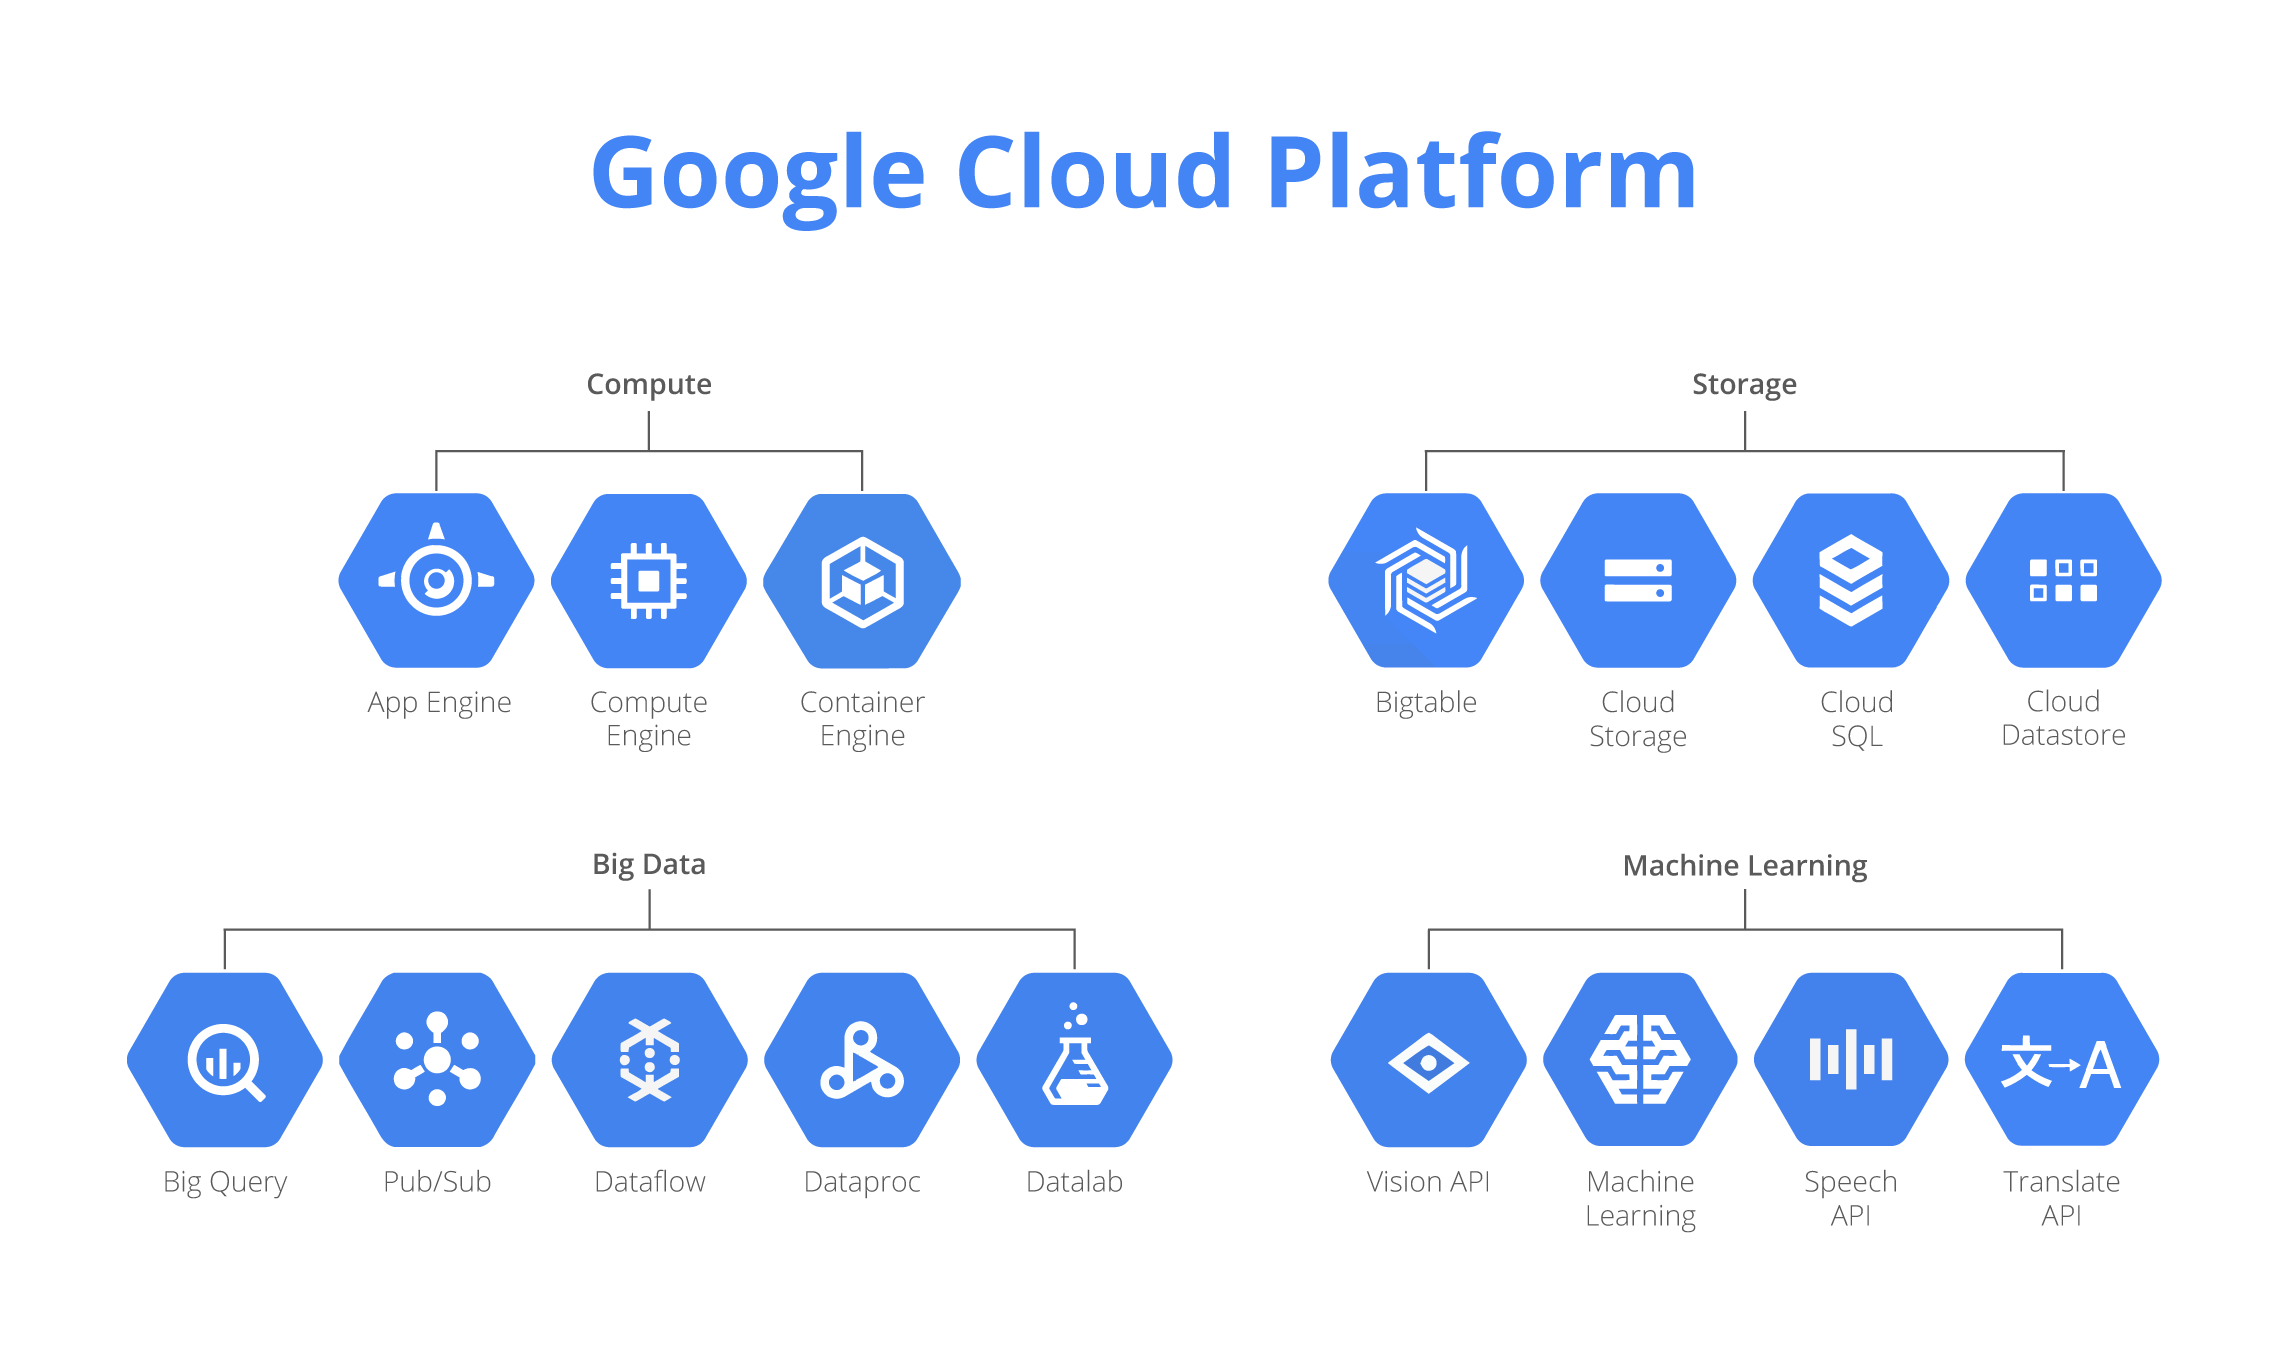
\includegraphics[height=8cm]{img/googlecloudproducts}
	\caption{Productos de Google Cloud.}
	\label{figura:googlecloudproducts}
\end{figure}

Google Compute Engine, o GCE es básicamente una infraestructura que permite levantar \textbf{máquinas virtuales} de forma escalable a las cuales se puede acceder via SSH, API, y más formas. Esta máquina virtual, a la hora de crearla, deja escoger qué tipo de memoria principal tiene, el sistema operativo y el número de CPUs (\textit{Central Processing Unit}) y TPUs (\textit{Tensor Processing Unit}); este último componente se emplea para los mecanismos de aprendizaje automático, que en este caso no aplica.

Como se menciona en la tabla \ref{tabla:caracteristicasgce}, en la cual podemos ver las características de la máquina virtual empleada para contener el simulador de diabetes, la IP es necesario que sea estática; se necesita que tanto el robot como la aplicación Java sepan dónde se encuentra el servicio en la nube en todo momento. \\

\begin{table}[!h]
	\begin{center}
		\begin{tabular}{|l|r|}
			\hline 
			\textbf{Característica} & \textbf{Descripción} \\ 
			\hline 
			Sistema operativo & Ubuntu 19.04 \\ 
			\hline 
			Memoria principal & 3,75 GB \\ 
			\hline 
			Memoria del disco & 10 GB \\ 
			\hline 
			CPU & 1 vCPU \\ 
			\hline 
			IP & Estática (34.76.240.69) \\ 
			\hline 
		\end{tabular} 
		\caption{Características de la máquina virtual de GCE}
		\label{tabla:caracteristicasgce}
	\end{center}
\end{table}

Se han levantado dos servicios dentro de la máquina virtual, para cada uno de los cuales debe entrarse por un puerto diferente. El primero es un \textit{broker} MQTT, el cual se explica en la sección  y el segundo el propio servidor para el simulador de diabetes. \\

\section{Servidor de diabetes}

Del proyecto anterior, se ha quitado la parte del simulador de diabetes y se ha movido a la máquina virtual de Google Compute Engine, como se ha comentado en otras secciones. Pero para acceder a él y poder manejarlo, antes debe superponerse una capa (API, \textit{Application Programming Interface}) para el manejo de peticiones entrantes. En este caso se ha decidido utilizar el modelo REST sobre un servidor HTTP.

\subsection{HTTP}
HTTP, o \textit{HyperText Transfer Protocol}, es el protocolo de red que permite la transferencia de documentos de hipermedia en la red, generalmente entre un navegador y un servidor aunque en este proyecto sea a través de una aplicación Python y Java, para que los humanos puedan leerlos. \\

Sobre las URLs de los servicios web se pueden hacer muchos tipos de operaciones, que son exactamente: GET, HEAD, POST, PUT, DELETE, TRACE, OPTIONS, CONNECT, PATCH, SEARCH, COPY, LOCK, UNLOCK, MOVE, MKCOL, PROPFIND, PROPPATCH, MERGE, UPDATE y LABEL. Se aprecia que los nombres son cuasi descriptivos por si solos. \\

Las peticiones y las respuestas de peticiones llevan una cabecera con metadatos para indicar por ejemplo si lo que va a recibirse está en formato XML, JSON... (Se llama MimeType), o el lenguaje de la respuesta, entre otras opciones de metadatos. Después de las cabeceras viene el cuerpo del mensaje en sí, que contiene la información solicitada o de petición. \\

También está en el protocolo el código de las respuestas. Según el código recibido quieren decir una cosa u otra, pero se agrupan en cinco tipos de formato de código:
\begin{itemize}
	\item Formato 1xx: Respuestas informativas. Indica que la petición ha sido recibida y se está procesando.
	\item Formato 2xx: Respuestas correctas. Es el resultado deseado.
	\item Formato 3xx: Respuestas de redirección. Indica que el cliente necesita realizar más acciones para finalizar la petición.
	\item Formato 4xx: Errores causados por el cliente. Indica que ha habido un error en el procesado de la petición a causa de que el cliente ha hecho algo mal.
	\item Formato 5xx: Errores causados por el servidor. Indica que ha habido un error en el procesado de la petición a causa de un fallo en el servidor.
\end{itemize}

\subsection{REST}
Como se menciona en este artículo \cite{PrincipiosREST}, REST fue presentado por primera vez en el 2000 por Roy Fielding en la Universidad de California. REST (\textit{Representational State Transfer}) es una arquitectura de programación pensada para servicios web, que se transfieren mediante HTTP. Ha desplazado enormemente a SOAP gracias a su sencillez de uso y de entendimiento. Sigue cuatro principios de diseño:
\begin{itemize}
	\item Utilice métodos HTTP de forma explícita: El cliente interactúa con el servidor únicamente con métodos HTTP mediante operaciones de crear, leer, actualizar y borrar, que para REST son:
		\subitem -- Para crear un recurso en el servidor hay que utilizar un POST.
		\subitem -- Para consultar un recurso hay que utilizar un GET.
		\subitem -- Para cambiar el estado de un recurso hay que utilizar un PUT.
		\subitem -- Para borrar un recurso hay que utilizar un DELETE.
	\item Sea sin estados: Un mensaje no tiene porqué depender de un mensaje anterior para que se entienda, sino que cada mensaje debe tener toda la información necesaria.
	\item Exponga los URIs (\textit{Uniform Resource Identifier}) como estructuras de directorios. 
	\item Transfiera XML, JavaScript Object Notation (JSON), o ambos.
\end{itemize}

\subsection{HTTP y REST en este proyecto}
Se ha decidido emplear HTTP y REST en este proyecto porque como se mencionaba antes, su uso es el más extendido hoy en día debido a su sencillez. \\

Como se aprecia, HTTP y REST por si solos no pueden entenderse, pues HTTP necesita guiarse por el patrón que marca REST y REST necesita que HTTP de cuerpo a su arquitectura. Así que se explican de manera conjunta. \\

Se ha seguido la estructura de las URIs como REST manda que se monte, es decir, como una estructura de directorios. Cuando se compone toda la URL, y se implementan los métodos, los puntos de acceso al servidor y sus respuestas son los que se indican en las tablas \ref{tabla:urishttpget} y \ref{tabla:urishttpput}. En esta tabla se ha recortado la URL y se ha dejado solamente la ruta hasta el recurso. La URL absoluta tiene el prefijo \url{http://34.76.240.69:8080}, que por ejemplo para acceder al recurso raíz (/) será \url{http://34.76.240.69:8080/}, o para acceder a /Hilo/, \url{http://34.76.240.69:8080/Hilo/}. Nótese que solamente se han empleado los métodos HTTP GET y PUT, pues solo se permiten operaciones de lectura y de actualización de recursos.

\begin{table}[!h]
\begin{center}
\begin{tabular}{|l|c|c|}
	\hline 
	\textbf{URL} & \textbf{GET} & \textbf{Respuesta}\\ 
	\hline 
	/ & Sí & Es para probar la conectividad, \\ 
	&& devuelve "Hello World".\\
	\hline 
	/Hilo/ & Sí & Devuelve el estado del hilo:\\ 
	&& PARADO, PAUSADO, CORRIENDO. \\
	\hline 
	/Simulador/Modo/ & Sí & Devuelve el modo actual del simulador.\\ 
	\hline 
	/Simulador/Glucosa/ & Sí & Devuelve la glucosa actual\\ 
	&& del simulador de diabetes.\\
	\hline 
	/Simulador/ & Sí & Devuelve, si lo tiene, el dato\\ 
	DatosSimulacion/&& de simulación que se ha enviado.\\
	\hline 
\end{tabular} 
\caption{Estructura de URIs y descripción de método HTTP GET sobre el servidor de diabetes.}
\label{tabla:urishttpget}
\end{center}
\end{table}

\begin{table}[!h]
	\begin{center}
		\begin{tabular}{|l|c|c|}
			\hline 
			\textbf{URL} & \textbf{PUT} & \textbf{Respuesta} \\ 
			\hline 
			/ & No & - \\ 
			\hline 
			/Hilo/ & Sí, acepta como & Si se ha podido aplicar  \\ 
			& parámetros PARADO, & la operación al hilo,\\
			& PAUSADO, CORRIENDO. & devuelve 200 OK,\\
			& sino respuesta 4xx. & \\
			\hline 
			/Simulador/Modo/ & Sí, admite los valores 1,2,3 & Si todo ha ido bien,\\ 
			&& 200 OK, sino 4xx. \\
			\hline 
			/Simulador/Glucosa/ & No & - \\ 
			\hline 
			/Simulador/ & Sí, admite un JSON & Si todo ha ido bien, \\ 
			DatosSimulacion/ & con los datos para & 200 OK, sino 4xx.\\
			& una nueva simulación. & \\
			\hline 
		\end{tabular} 
		\caption{Estructura de URIs y descripción de método HTTP PUT sobre el servidor de diabetes.}
		\label{tabla:urishttpput}
	\end{center}
\end{table}

Para hacer real esta estructura, esta \textit{API}, hay que programarlo en alguna tecnología. Se escoge \textbf{Python 2.7}, para mantener la coherencia con el resto del proyecto, el código en NAO, que está obligado a ser en Python 2.7 también, como se explica más adelante. Antes estaba escrito en C++, pero existen utilidades más modernas y moldeables en Python, por lo que se aprovecha el gran cambio que va a sufrir el simulador para convertirlo a un lenguaje más flexible. \\

Primero, se utiliza un \textbf{servidor WSGI en el puerto 8080} para que la aplicación Python escuche las peticiones entrantes. WSGI significa \textit{Web Server Gateway Interface} y es el conjunto de servidores web que reenvían las peticiones a las aplicaciones web escritas en Python. Tienen dos partes: la primera la parte del servidor en si, que en este caso está construida sobre Nginx, y la segunda, que es la implementación de la API REST en sí. De las posibles opciones que existen en Python, se ha escogido \textbf{gevent}, cuyo sitio oficial se encuentra en \cite{WSGIGevent}. Crear una aplicación web con WSGI es muy sencillo y más aún si se combina con Flask. \\

\textbf{Flask} es un \textit{web framework}, lo que significa un conjunto de herramientas y librerías que hacen muy simple estructurar una aplicación web. Su mayor competidor es Django, pero es más recomendable utilizar Flask junto con Python, por no mencionar que es mucho más simple utilizar Flask. Dado que la API construida no tiene más que un dos clientes, tampoco es necesario algo muy potente, así que la simpleza se valora más. Añadido a Flask, hay una extensión llamada \textbf{Flask RESTful} \cite{FlaskRESTful} que abstrae un método Flask convencional para convertirlo en una serie de operaciones sobre un recurso de la jerarquía de URIs.\\

Juntando la máquina de Google Compute Engine y las tecnologías para montar la API REST --WSGI y Flask--, se consigue hacer la puerta de entrada para poder interactuar con el simulador, el cual está encapsulado en un hilo de ejecución. Mediante la API REST se puede activar, pausar, detener o reanudar la ejecución del hilo de ejecución del simulador, así como consultar la glucosa actual en cada momento o enviar datos para simular. Pero lo que falta por convertir es la librería que hace el cálculo de las ecuaciones diferenciales.

\section{Sistema MQTT}

\subsection{Introducción a MQTT}

MQTT significa \textit{Message Queue Telemetry Transport}. Es un protocolo del tipo publicador/suscriptor, extremadamente simple y ligero, diseñado para dispositivos limitados o con poco ancho de banda. Los principios de diseño son minimizar el ancho de banda de la red y los requisitos de recursos del dispositivo al mismo tiempo que se intenta garantizar la confiabilidad y cierto grado de garantía de entrega. Estos principios también hacen que el protocolo sea ideal para el emergente mundo de dispositivos conectados <<máquina a máquina>> (M2M) o <<Internet de las cosas>> (IoT), y para aplicaciones móviles donde el ancho de banda y la energía de la batería son muy importantes. Además, la versión 3.1.1 se encuentra certificada en la ISO/IEC PRF 20922 \cite{MQTTISO}. \\

En MQTT hay dos tipos de agentes que intervienen: 
\begin{itemize}
	\item El \textbf{\textit{broker}}: Es el servidor que contiene las colas de mensajes. Los clientes depositan mensajes en las colas (\textit{publican} estos mensajes) de forma que otros clientes reciben estos mensajes encolados. Solo existe un broker por cada sistema MQTT.
	\item \textbf{Clientes}: Puede haber tantos clientes como se desee. Son los que generan los mensajes que envían al broker, y el broker se encarga de distribuirlos a los clientes que pertoque. 
\end{itemize}

El hecho de enviar un mensaje al broker se llama \textbf{publicar}, y para que un cliente pueda recibir los mensajes, debe \textbf{estar suscrito} a ellos. La operación de recepción de un mensaje es asíncrona, pues se reciben los mensajes y se ejecuta una llamada como consecuencia (\textit{callback}). Para identificar a qué suscriptores pertenece cada mensaje, se emplean unas etiquetas, que pueden contener niveles de jerarquía, al estilo de los directorios en sistemas operativos. Por ejemplo, si se publica un mensaje \textit{topic1/topic2}, y un suscriptor indica que desea recibir los mensajes sobre esa etiqueta, así se hará. Pero hay dos carácteres especiales. Supóngase la etiqueta de ejemplo anterior: 
\begin{itemize}
	\item \textbf{\#}: Si un cliente decide suscribirse a \textit{topic1/\#}, recibirá todos los mensajes cuya etiqueta comience por \textit{topic1/}.
	\item \textbf{+}: Si algún suscriptor decide suscribirse a \textit{+/topic2}, recibirá todos aquellos mensajes que comiencen por cualquier etiqueta en el primer nivel, pero que en el segundo nivel se llamen \textit{topic2}.
\end{itemize} 

Puede observarse un ejemplo gráficamente en la figura \ref{figura:mqttexplanation}.

\begin{figure}[!h]
	\centering
	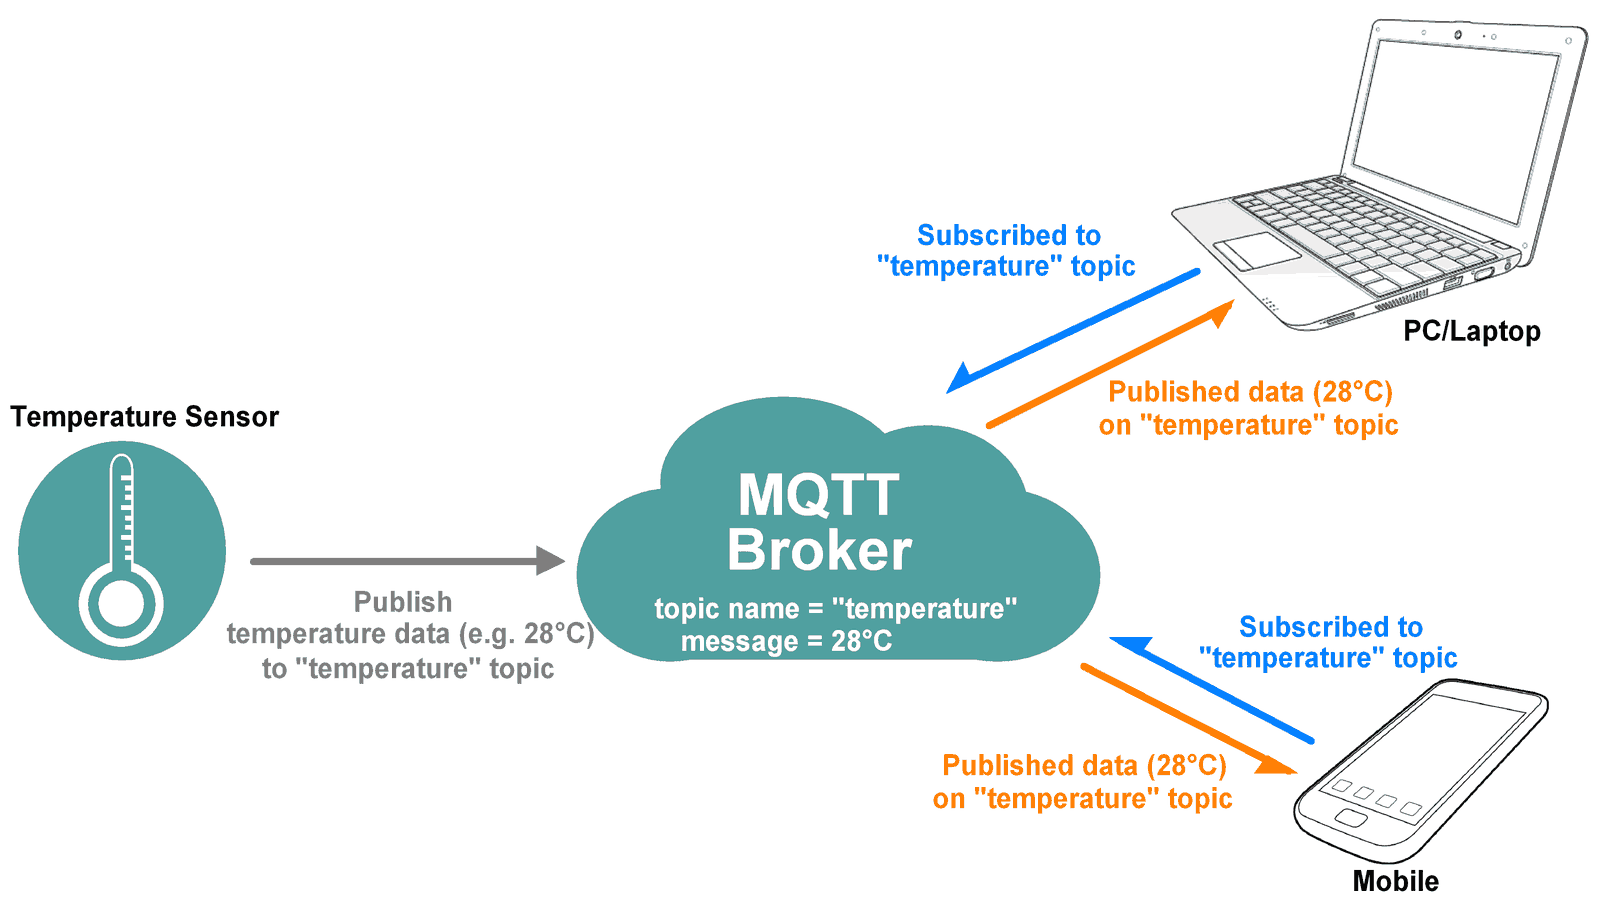
\includegraphics[height=8cm]{img/mqttexplanation}
	\caption{Ejemplo del funcionamiento de MQTT.}
	\label{figura:mqttexplanation}
\end{figure}

Existen muchas implementaciones de MQTT: Paho MQTT, Mosquitto, HiveMQ, Adafruit IO, las cuales son las más famosas, pero hay más. Muchas de ellas son de código abierto, otras no, están desarrolladas por diversas empresas o universidades y demás características que se pueden observar en este enlace \cite{MQTTComparison}. \\

\subsection{MQTT en este proyecto}

Para este proyecto se han empleado dos tipos de MQTT del mismo proveedor, Eclipse, que ha desarrollado M2Mqtt, Mosquitto y Paho MQTT. El primero, \textbf{Mosquitto}, se ha utilizado para instalar el \textbf{broker} en la máquina virtual. Dado que Mosquitto es la única de las tres implementaciones de Eclipse que tiene un broker, no había más opción que instalarlo. Para cliente, solamente tiene integración con el lenguaje de programación C, así que se desarrollan los \textbf{clientes} con \textbf{Paho MQTT}, que es el segundo componente, pues tiene un nivel de compatibilidad muy alto -- se adapta a C, C++, Java, JavaScript, Python y Go. \\

Dado que el broker Mosquitto se implementa en la máquina virtual, que lleva Ubuntu 19.04 como sistema operativo, la fuente de instalación es los propios repositorios de Ubuntu. Se instala sobre el puerto \textbf{TCP 1883} y se emplea autenticación de usuario y contraseña. La conexión es no-TLS (\textit{Transport Layer Security}), pero si se quisiera una conexión cifrada (TLS) debería instalarse en el puerto 8883. Para activar el servidor no hay que hacer más que activar un servicio con \textit{systemctl}. \\

Los clientes MQTT están tanto en el código NAO como en la aplicación Java, y ambos tienen detallados su funcionamiento en sus secciones pertinentes. \\

Los mensajes que se envían llevan una etiqueta, o tema, cuyo detalle de qué significa se encuentra en la tabla \ref{tabla:topicsmqtt}. \\

La intención al haber empleado este sistema es sustituir la conexión TCP que enviaba mensajes periódicamente por una conexión asíncrona como es ésta. Podría haberse empleado también el sistema HTTP que hay montado para la simulación de diabetes y que los clientes si desean saber el estado de una variable, pueden consultarla periódicamente (mecanismo que se conoce como \textit{polling}, o muestreo de una variable), pero supone un problema de coste; se saturaría el sistema tras atender tantas peticiones periódicas y además la intención es aligerar computacionalmente el sistema, y ésta no es la manera. \\

\begin{table}[!h]
\begin{center}
\begin{tabular}{|c|c|}
	\hline 
	\textbf{Topic (tema)} & \textbf{Descripción} \\ 
	\hline 
	hilos & Topic, o tema, que recoge información \\
	& sobre el estado de los hilos que \\
	& funcionan con MQTT, es decir, los hilos \\ 
	& excluyentes. Esta información viene con \\ 
	& un separador en un texto, que es del formato \\ 
	& \textit{hilo,estado}, siendo hilo el nombre \\
	& del hilo involucrado y estado una cadena \\ 
	& de caracteres con los posibles valores: \\ 
	& PARADO, CORRIENDO, PAUSADO. \\ 
	\hline 
	interfaz/\# & Es un tema padre, que son aquellos \\
	& datos que deben ser visibles para el \\ 
	& usuario mediante una interfaz. \\
	\hline 
	interfaz/ventanaescenario & Se recoge bajo este subtopic \\ 
	& aquellos datos que deben mostrarse \\
	& de manera auxiliar para que el usuario \\
	& tenga más información del hilo excluyente \\
	& Escenario, que es complejo. \\ 
	\hline 
	nao/\# & Siendo este tema un tema padre, se \\
	& recoge bajo este tema toda aquella \\
	& información que tenga que ver con la \\
	& configuración de acciones sobre el robot \\
	& NAO. \\ 
	\hline 
	nao/decir & Bajo este subtema o subtopic se envían \\
	& órdenes de habla para que diga con voz \\
	& la frase recogida bajo este tema. \\ 
	\hline 
	nao/mover & Bajo este subtema o subtopic se envían \\
	& órdenes de acciones con movimiento. \\
	& Estas pueden ser: Pincharse, Sentarse, \\
	& Parada, Comer, MedirGlucosa, Correr. \\ 
	\hline 
	nao/leds & En este subtema se envían órdenes de \\
	& encendido de leds según si se quiere \\
	& encender o apagar la tonalidad de los \\
	& leds de los ojos. Viene en formato \\
	& \textit{color,onoff} y color puede ser verde, \\
	& rojo o azul, y onoff simplemente \\
	& on o off. \\ 
	\hline 
	nao/exacpalabra & En este subtema se reciben órdenes de \\
	& establecimiento del mínimo de la exactitud \\
	& de la palabra a la hora de reconocer voz. \\
	& Es decir, qué mínima tiene que haber \\
	& para dar una palabra por reconocida. \\ 
	\hline 
\end{tabular} 
\caption{Temas utilizados en este proyecto y su significado.}
\label{tabla:topicsmqtt}
\end{center}
\end{table}

\newpage
\section{Librería para el cálculo diferencial}

Lo último necesario para terminar de migrar el simulador de diabetes a una aplicación web Python es adaptar la librería de cálculo diferencial. Tal como se menciona en la introducción de este proyecto, se sigue un modelo de simulación según Hovorka que emplea ecuaciones ODE (ecuaciones diferenciales ordinarias). En el simulador del anterior proyecto se emplea la librería Alglib, hecha para C++. Al convertir la aplicación a Python, es necesario cambiar también la librería de cálculo. \\

Alglib \cite{Alglib} tiene una licencia comercial y otra gratuita, esta última para fines no comerciales como es esta aplicación. Empleando la opción gratuita, existe un \textit{wrapper} o una aplicación que engloba a la librería construida para C++, para que pueda utilizarse en Python. En un principio se había pensado en emplear esta opción para respetar los cálculos iniciales pero supone una limitación a la hora de actualizar la librería de la aplicación Python. Esta librería para actualizarse depende de que se actualice su código interno C++ y luego el \textit{wrapper} para ésta. \\

Por lo tanto se ha migrado la librería de cálculo a \textbf{SciPy} \cite{Scipy}, un módulo Python para cálculo matemático entre otras funciones, cuyo uso está muy extendido. De hecho, de sus paquetes centrales, existen unos que son muy famosos como NumPy, IPython o Matplotlib.

\chapter{Código en NAO}

\section{Problemas con el código anterior}

En el anterior proyecto, el código NAO incluía toda la lógica necesaria para que el robot estuviera en marcha. Como es el objetivo de este trabajo aligerar carga, se ha reducido la cantidad de clases que hay en el código anterior, cuyas relaciones se pueden ver en la figura \ref{figura:clasesnaoprevio}. Hay doce clases y están escritas en C++, cuya compilación es muy laboriosa, ya que emplea una serie de herramientas, algunas de NAOqi, que encorsetan demasiado el proyecto. NAOqi es el \textit{framework}, o conjunto de librerías y programas, en el que consiste el programa principal del robot y que lo controla. Estas herramientas que se emplean para la compilación son:
\begin{itemize}
	\item Compilación con Cmake, una herramienta que ayuda a la compilación de código en C++, para automatizar este proceso.
	\item Qitoolchain es el conjunto de compilador cruzado, enlazador de librerías y otras funciones, necesarias para montar un ejecutable.
	\item NaoqiSDK es el conjunto de clases, métodos y demás elementos para construir el código necesario para acceder a las funciones del robot.
	\item Qibuild es la herramienta para construir un proyecto como NAO espera.
\end{itemize}

\begin{figure}[!h]
	\centering
	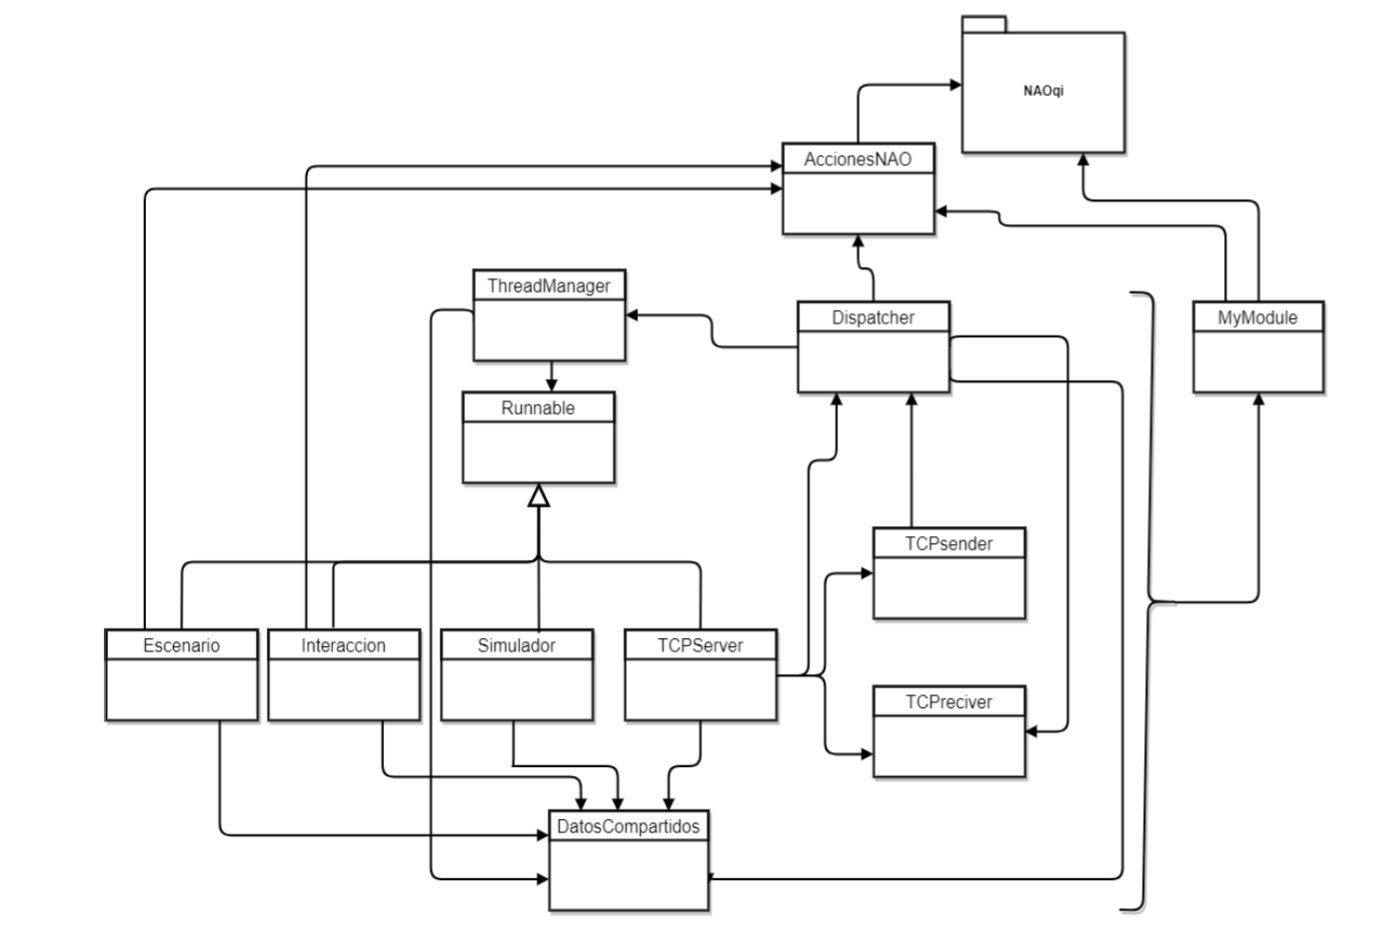
\includegraphics[height=10cm]{img/clasesnaoprevio}
	\caption{Clases de anterior proyecto en el código de NAO.}
	\label{figura:clasesnaoprevio}
\end{figure}

Como puede verse en esta URL \cite{C++Desaconsejado} de la propia Aldebaran, la empresa propietaria de los robots NAO, se desaconseja el uso del lenguaje C++ si no se tiene un gran conocimiento de la compilación cruzada. Pero mayormente el problema reside en que no se puede añadir una librería de terceros de forma sencilla porque las herramientas de NAOqi restringen mucho su uso y resulta un proceso demasiado complejo.

\section{Código actual}

\subsection{Cambio a Python} \label{CambioPython}

Para el código nuevo que se aloja en el robot NAO se ha decidido transformarlo en Python porque resulta mucho más sencillo montar un programa funcional que con C++ y es también mucho más fácil incluir librerías de terceros --a pesar de que tampoco es sencillo del todo en Python debido a unas limitaciones que tiene NAO que se verán más adelante. Se ha aprovechado el hecho de que el programa iba a sufrir una transformación muy grande de todos modos para modernizarlo un poco más. Además, Aldebaran aconseja su uso también en su web \cite{ProgrammingLanguages}, justificando que Python es más compatible (en la imagen \ref{figura:comparativalenguajes} se ve la comparativa) con otras aplicaciones suyas como \textit{Choreographe}, que en este proyecto no se utiliza pero si es necesario hacerlo en futuras ocasiones será de provecho.

\begin{figure}[!h]
	\centering
	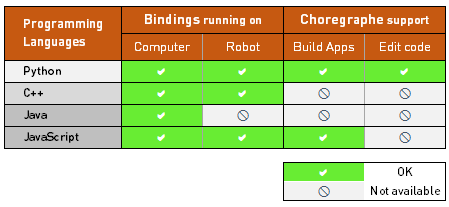
\includegraphics[height=6cm]{img/supported_language}
	\caption{Tabla comparativa de lenguajes de programación en NAO.}
	\label{figura:comparativalenguajes}
\end{figure}

La versión de Python que dispone NAO es únicamente la versión \textbf{Python 2.7}. Esta es la versión con la que se permite conectar a los llamados \textit{proxies}, que no son más que las llamadas a los componentes \textit{hardware} como los motores o las cámaras para que ejecuten sus funciones. 

\newpage
\subsection{Clases del código en NAO}

Se ha conseguido reducir el número de clases de doce a siete, ya que sin el hilo del simulador ni el hilo TCP se perdía mucho grueso de la ejecución y por lo tanto puede reducirse más de lo esperado. Si antes el diagrama de clases era como en la figura \ref{figura:clasesnaoprevio}, en este proyecto el diagrama de clases es como en la figura \ref{figura:naoprogramaactual}.

\begin{figure}[!h]
	\centering
	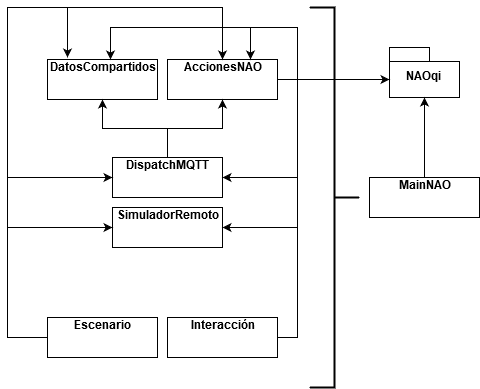
\includegraphics[height=8cm]{img/clasesnaonuevo}
	\caption{Diagrama de clases del código de NAO actualmente.}
	\label{figura:naoprogramaactual}
\end{figure}

Las clases nuevas implementadas son \textbf{DispatchMQTT} y \textbf{SimuladorRemoto}, las cuales llevan los clientes de MQTT y HTTP para conectar con el simulador remoto y el \textit{broker} MQTT. Pero el resto de clases se merecen una observación porque la mayoría ha sufrido un cambio considerable:
\begin{itemize}
	\item \textbf{DatosCompartidos}: Se ha reducido la cantidad de datos compartidos, ya que al cambiar las comunicaciones, la mayor parte ya no se utiliza. Además, se ha añadido la gestión de los hilos excluyentes a esta clase, para que gestione cuál de los dos hilos está en activo: si Escenario o Interacción.
	\item \textbf{AccionesNAO}: Se ha mantenido la lógica de esta clase prácticamente igual que en C++, pero pasada a Python. Se comunica directamente con los \textit{proxies} de NAOqi para hacer movimientos, escuchar palabras y decir palabras, entre otras funciones.
	\item \textbf{DispatchMQTT}: Es una clase nueva que emplea la librería externa \textit{Paho MQTT} que contiene el cliente MQTT mediante el cual está a la espera de nuevos mensajes que le pueden llegar desde el \textit{broker}, en el Google Compute Engine. Cuando reciba un mensaje, ejecutará una \textit{callback}, de forma que así se ahorra un hilo al ejecutar tareas asíncronamente. De igual forma puede publicar mensajes al \textit{broker} para que los reciba otro cliente suscrito a un tema. Estos casos pueden ocurrir en cuanto la interfaz Java ordene al hilo Escenario o Interacción detenerse, arrancar o pausarse. También puede ocurrir que si ningún hilo excluyente está activo, puede ordenar acciones simples como decir una frase, hacer un movimiento simple, etcétera.
	\item \textbf{SimuladorRemoto}: Contiene el cliente HTTP que envía peticiones al servidor REST que está montado en el Google Compute Engine. Contiene las llamadas para ejecutar los métodos de las tablas \ref{tabla:urishttpget} y \ref{tabla:urishttpput}, que arranca, para o pausa el simulador de diabetes y además puede consultar la glucosa y publicar datos de simulación. Estos métodos se utilizan combinados con el objeto Escenario, cuando se le ordena comer o hacer ejercicio, por ejemplo. Para ello se ha empleado la librería \textit{requests}, una librería propia de Python.
	\item \textbf{Interacción}: Es uno de los dos hilos excluyentes. La lógica de esta clase se ha alterado mínimamente, pues es una clase en la que simplemente se reciben órdenes verbales y se responde con una acción.
	\item \textbf{Escenario}: El otro de los dos hilos excluyentes. Es similar a Interacción, pero es más complejo. Consta de dos fases. La fase 2, tiene pocas órdenes verbales que atiende, pero aún así tiene en cuenta la glucosa que tiene en dicho instante y toma medidas correctoras si fuera necesario. Por ejemplo, si hay una situación de glucosa muy alta, se pincha insulina de urgencia. La fase 3 es como la fase 2 pero más compleja, pues tiene estados dentro de la fase, muchas más órdenes posibles, comportamientos correctos e incorrectos, entre otras cosas.
	\item \textbf{MainNAO}: La clase principal. Se ha cambiado la lógica porque principalmente, se ha modificado toda la arquitectura de clases y hay que construirlo de otro modo todo, y en segundo lugar, porque no es la misma inicialización de clases para Python que para C++. En Python es mucho más sencillo.
\end{itemize}

Las clases que han desaparecido han sido la interfaz \textit{Runnable}, pues solamente la implementarían dos clases, y dos métodos de una línea cada clase, así que se ha implementado directamente -- además que en C++ era necesario implementar una interfaz que unificara los tipos de los objetos y en Python esto no es necesario, al ser un lenguaje no tipado. También ha desaparecido \textit{TCPServer}, \textit{TCPReceiver} y \textit{TCPSender}, porque se han sustituido por las clases cliente de HTTP y MQTT. Se ha eliminado \textit{Simulador} porque como se ha mencionado repetidamente, se ha convertido en un servicio web. La clase \textit{ThreadManager} se ha integrado con DatosCompartidos, porque al eliminar los hilos que atienden las conexiones TCP y el Simulador, quedan solamente dos hilos excluyentes que gestionar, y de paso también \textit{Dispatcher} porque era una clase que unificaba las clases TCP para lanzar hilos excluyentes y no excluyentes. \\

En el capítulo 5 se explica bien el funcionamiento de esta parte del proyecto interrelacionada con las demás partes, porque por si sola carece de significado. Necesita que las demás clases la activen.

\chapter{Aplicación Java}

El cliente Java ha sufrido un cambio mínimo. Lo más destacable es la sustitución de la clase TCP por los mecanismos de comunicación nuevos, MQTT y HTTP. Para MQTT, se ha empleado \textbf{Paho MQTT}, el cliente creado por Eclipse y para HTTP se utilizado la librería propia de Java \textbf{java.net}. El diagrama de clases queda como en la imagen  \ref{figura:clasesjava}, y las nuevas clases incluidas son \textit{ConectaGCloud} y \textit{ConectaMQTT}.

\begin{figure}[!h]
	\centering
	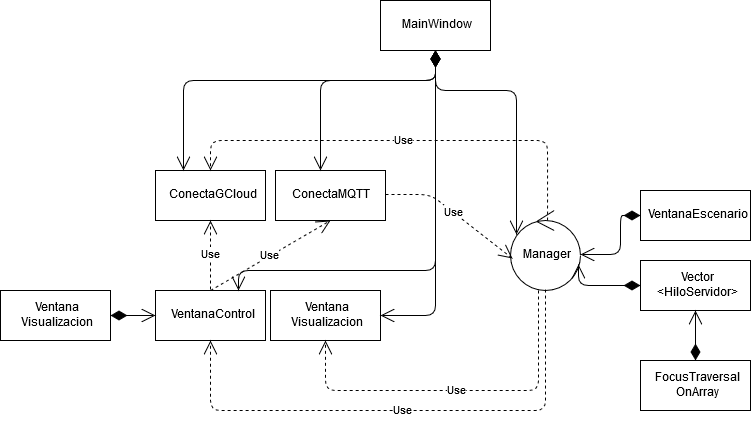
\includegraphics[height=9cm]{img/ClasesJava}
	\caption{Diagrama de clases del cliente Java.}
	\label{figura:clasesjava}
\end{figure}

A diferencia de la sección del código en NAO, en la que se explicaba cada clase cómo se había transformado, en esta parte no va a desglosarse el funcionamiento, pues la lógica del programa es prácticamente la misma a excepción de las dos clases nuevas que se han añadido.

\section{MQTT en la aplicación Java}

Se aloja en la clase ConectaMQTT. Emplea para ello el cliente de Paho MQTT, una librería de terceros, como se ha mencionado antes, y las funciones que realiza son, como en el código NAO, dos:
\begin{itemize}
	\item \textbf{Publicar mensajes}: Está configurado para publicar al \textit{broker} MQTT mensajes tanto de estado de hilos (apagado, encendido o pausado), como también puede ejecutar órdenes simples que van directas a la clase \textit{AccionesNAO}, en caso de que no haya ningún hiloExcluyente corriendo, para que se mueva, hable, encienda unos leds, entre otros.
	\item \textbf{Suscribirse a mensajes}: Está suscrito a los mensajes del estado de los hilos, para recibir si se ha apagado algún hilo, y al estado del hilo Escenario para en el caso de que esté activo el hilo mencionado, transmita el estado en el que se encuentra. Al final esto es para obtener más trazabilidad, pues el hilo de Escenario es bastante complejo.
\end{itemize}

\section{HTTP en la aplicación Java}

Las conexiones HTTP están implementadas en la clase \textit{ConectaGCloud}. Se realizan peticiones HTTP a las URLs especificadas en las tablas \ref{tabla:urishttpget} y \ref{tabla:urishttpput} mediante el paquete propio de Java, \textit{java.net}, como se ha mencionado previamente.\\

Hay dos peticiones que se ejecutan cada segundo de forma \textbf{periódica}. La primera es para consultar el nivel de glucosa que actualmente marca el simulador de diabetes y ubicar el dato en la gráfica del nivel de glucosa. La segunda es para consultar el estado del hilo del simulador, es decir, para consultar si se encuentra apagado, pausado o en activo. Así lo marcará en un color en la interfaz, en el apartado de los hilos. \\

Las otras llamadas, las que no son periódicas, sino \textbf{esporádicas}, responden a esta serie de acciones:
\begin{itemize}
	\item Verificar que el servicio web del simulador está en marca mediante una consulta a la URL padre. Si responde correctamente, dejará arrancar la aplicación Java, y sino, lanzará un mensaje de error.
	\item Operaciones sobre la URL de /Hilo/ para detener, pausar o activar el hilo que simula los niveles de glucosa.
	\item Envío de parámetros de simulación nuevos. Esto en la interfaz se muestra de manera que hay dos órdenes predefinidas, una de comer, para que aumente la glucosa, y otra orden de deporte, para que baje. Pero también existe la posibilidad de enviar una orden personalizada con el nivel de insulina inyectada, la cantidad de comida ingerida y deporte si es que lo hay.
	\item Establecimiento del modo de simulación, siendo el modo de simulación la lentitud o rapidez con la que se simula el comportamiento del páncreas.
\end{itemize}

\chapter{Relación entre los componentes}

\section{Jerarquía de los componentes}

\begin{figure}[!h]
	\centering
	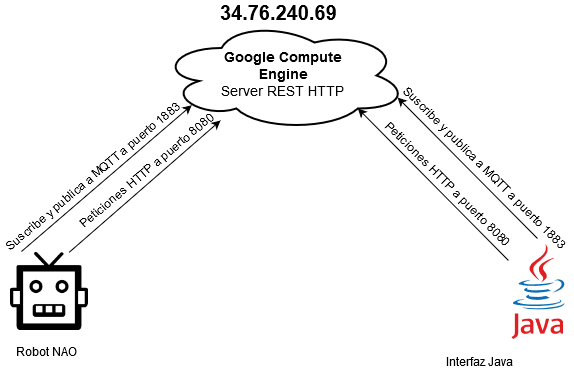
\includegraphics[height=9cm]{img/Conexion}
	\caption{Partes del proyecto conectadas.}
	\label{figura:conexionpartes}
\end{figure}

Las partes de este proyecto tienen dos niveles de jerarquía. El primero, el \textbf{servidor}, es el ocupado por la parte en Google Compute Engine, la máquina virtual. En ella se aloja tanto el \textit{broker} MQTT como el servidor WSGI que contiene el servidor REST. Atiende peticiones en el puerto 1883 para MQTT y en el puerto 8080 para las peticiones REST. Tiene una capacidad de cómputo alta, y es escalable en caso de que el número de peticiones creciera, pero no es el caso porque el proyecto por el momento no puede tener más clientes. Su dirección IP debe ser fija, que lo es, para que aunque el robot y la aplicación cambien de red y por lo tanto se les asigne otra IP, puedan saber en todo momento donde deben referirse para obtener los servicios deseados.\\

La otra es la parte \textbf{cliente}, que la constituyen la aplicación Java y el robot NAO. La \textbf{aplicación Java} básicamente se encarga de enseñar al usuario el estado del robot, así como un panel de control para manejar el estado del simulador y lanzar órdenes al robot. El \textbf{robot NAO} es el receptor de las órdenes que lanza la interfaz Java, y a la vez consulta el estado del simulador para actuar en consecuencia durante la ejecución de los hilos. \\

En la imagen \ref{figura:conexionpartes} se aprecia la relación explicada en los párrafos anteriores.

\section{Traza de ejecución}

En esta sección se cuenta cuál es el flujo de llamadas al servicio web y \textit{broker} por el que pasan las aplicaciones, y cual es la respuesta que generan, de forma que se lleva a cabo una ejecución correcta. \\

Suponiendo que la máquina virtual está activa y los servicios que contienen MQTT y REST se han levantado correctamente, primero \textbf{se arranca la aplicación Java}. Se muestra en ella la IP de la máquina virtual de Google Compute Engine por defecto, que como es estática, será la que hay escrita por defecto porque n va a cambiar, como se aprecia en la imagen \ref{figura:mainwindow}. Al pulsar el botón \textit{Conectar}, se hace una llamada \textbf{GET HTTP a http://34.76.240.69:8080/}, y si es exitosa, es decir, que el código de respuesta es \textbf{200 OK}, se procederá a los siguientes pasos en la aplicación. En caso de que no lo sea, se lanza un mensaje de error mediante un diálogo indicando que el Google Compute Engine no está disponible.

\begin{figure}[!h]
	\centering
	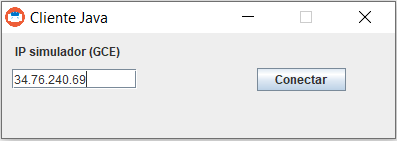
\includegraphics[height=4cm]{img/mainwindow}
	\caption{Ventana de arranque de la aplicación Java.}
	\label{figura:mainwindow}
\end{figure}

En este momento, si la llamada ha resultado correcta, se ejecutan una serie de pasos nuevos:
\begin{itemize}
	\item Se crea el cliente MQTT y se asocia a los topics que quiere suscribirse, que son \textbf{hilos} e \textbf{interfaz/ventanaescenario}.
	\item Se crea \textit{Manager}, que es una clase que ejecuta un hilo en el cual se consulta periódicamente al simulador vía HTTP cuál es su glucosa actual (\textbf{GET HTTP http://34.76.240.69:8080/Simulador/Glucosa/}), que devolverá un número decimal, y cuál es el estado actual del hilo del simulador (\textbf{GET HTTP http://34.76.240.69:8080/Hilo/}), que devolverá \textit{CORRIENDO}, \textit{PARADO} o \textit{PAUSADO}.
	\item Se crea \textit{VentanaControl}. En la ventana de control, como se aprecia en la figura \ref{figura:ventanacontrol1}, aparece una interfaz en la cual pueden ejecutarse una serie de órdenes hacia el robot -- pero que como todavía no está en marcha, aunque se envíen no se recibirán y se van a perder. Lo más relevante de esta vista es el panel de la derecha, que aparece SIMULADOR en rojo que significa que se encuentra detenido.Esto lo provoca la respuesta del simulador desde la llamada GET al estado del hilo.
	\item Se crea \textit{VentanaSimulacion}, como se ve en la figura \ref{figura:ventanavisualizacion1}. En esta gráfica se pintan los resultados de la llamada GET a la URL de glucosa del simulador. En el caso de recibir -1000, se indica que el simulador está detenido, como es el caso de la figura, y si se recibe -999, significa que el simulador está pausado. En caso distinto, se pintaría la gráfica con el histórico de valores de glucosa obtenidos del simulador de diabetes.
\end{itemize}

\begin{figure}[!h]
	\centering
	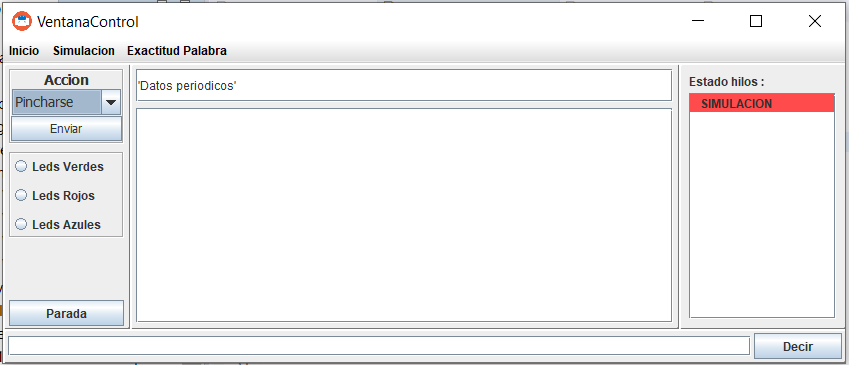
\includegraphics[height=6cm]{img/ventanacontrol1}
	\caption{Ventana de control al iniciar la aplicación Java.}
	\label{figura:ventanacontrol1}
\end{figure}

\begin{figure}[!h]
	\centering
	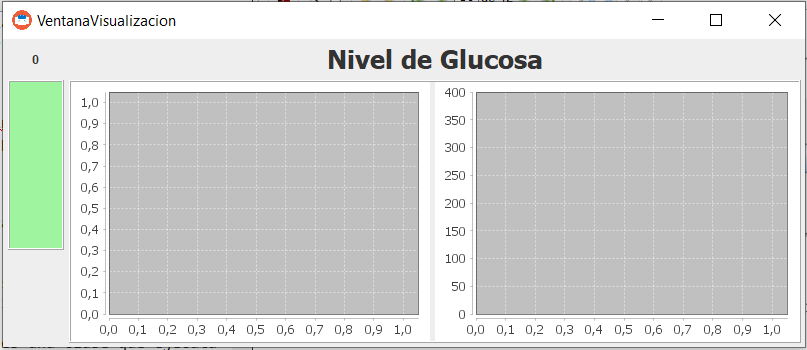
\includegraphics[height=6cm]{img/ventanavisualizacion1}
	\caption{Ventana de visualización del nivel de glucosa al iniciar la aplicación Java.}
	\label{figura:ventanavisualizacion1}
\end{figure}

El siguiente paso es \textbf{encender el robot}, que ejecuta el programa en Python. Lo primero que hace es suscribirse en el \textit{broker} MQTT a todos los subtemas que hay debajo de nao/, mediante la nomenclatura \textbf{nao/\#}, y a \textbf{hilos}. Crea las clases con hilos excluyentes -- Escenario e Interaccion -- con los hilos en reposo, y  \textbf{publica en <<INTERACCION,PARADO>> y <<ESCENARIO,PARADO>> en el tema <<hilos>>}. Cuando termina de publicar a MQTT, arranca el simulador mediante la orden \textbf{PUT HTTP http://34.76.240.69:8080/Hilo/, con el parámetro <<CORRIENDO>>}. De este modo, en la ventana de control se refleja con el color verde sobre simulador señalizando que el hilo ya se encuentra en marcha, y en la ventana de visualización ya se empieza a ver el progreso de la simulación de la glucosa. Además, al estar la aplicación Java suscrita a \textit{hilos}, recibe el mensaje de los hilos, y los añade a la lista de hilos en color rojo porque están parados. Se aprecia lo descrito en las imágenes \ref{figura:ventanacontrol2} y \ref{figura:ventanavisualizacion2}.

\begin{figure}[!h]
	\centering
	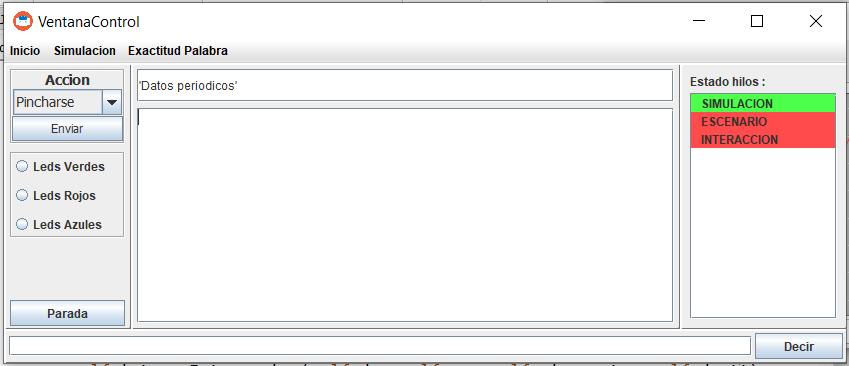
\includegraphics[height=6cm]{img/ventanacontrol2}
	\caption{Ventana de control en Java al haber iniciado el código de NAO.}
	\label{figura:ventanacontrol2}
\end{figure}

\begin{figure}[!h]
	\centering
	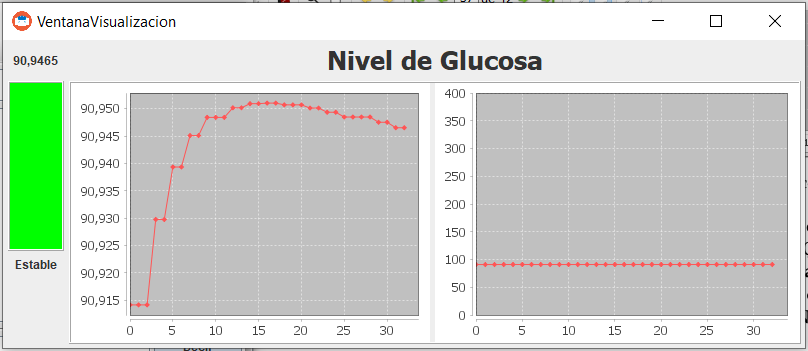
\includegraphics[height=6cm]{img/ventanavisualizacion2}
	\caption{Ventana de visualización en Java del nivel de glucosa al haber arrancado el simulador desde NAO.}
	\label{figura:ventanavisualizacion2}
\end{figure}

Con los hilos excluyentes apagados pueden ejecutarse órdenes simples como decir una frase escribiéndola en el cuadro de texto de debajo de la ventada de control, que publicaría el mensaje con la frase a pronunciar bajo el topic MQTT \textbf{nao/decir}, enviar acciones con el menú desplegable de la izquierda de ventana de control, que publica la acción en MQTT con el tema \textbf{nao/mover}, y así. En cambio, si se desea enviar una simulación de acción mediante la interfaz, en la opción del menú superior \textit{Simulación}, se enviará un \textbf{PUT HTTP http://34.76.240.69:8080/Simulador/DatosSimulacion/} con los datos en JSON de si hay bolo de comida, si se ha inyectado insulina y de si se ha hecho deporte. \\

Cuando se decide arrancar un hilo excluyente, se hace seleccionando un hilo de la ventana de control y mediante menú contextual, se selecciona \textit{Arrancar}. Esto genera una publicación <<ESCENARIO,CORRIENDO>> -- por ejemplo -- al tema \textbf{hilos de MQTT} que el robot NAO recibe mediante suscripción, y activa el hilo de lo seleccionado. \\

Supóngase que se ha activado el hilo Escenario, que es similar a Interacción pero con más actividad. Este hilo tiene un bucle infinito que solamente se detiene si desde la interfaz Java se selecciona el hilo y se pulsa mediante menú contextual la opción "Parar", que publica <<ESCENARIO,PARADO>> al tema \textbf{hilos de MQTT}. Pero durante su ejecución, el hilo primero consulta el nivel de glucosa mediante \textbf{GET HTTP http://34.76.240.69:8080/Simulador/Glucosa/}, y actúa en consecuencia. Si la glucosa tiene niveles extremos y se debe tomar medidas de urgencia, puede enviar él solo parámetros de simulación, para tomar comida urgentemente o pincharse insulina. Estas órdenes de simulación se envían de forma JSON en \textbf{PUT HTTP http://34.76.240.69:8080/Simulador/DatosSimulacion/}. En cambio si la glucosa tiene niveles dentro de un rango asumible, se gestiona según las órdenes que recibe de la persona que habla al robot. Paralelamente, este hilo concretamente publica a cada iteración el estado de las variables de control bajo el \textbf{topic MQTT interfaz/ventanaescenario}, de manera que la interfaz Java lo recoge porque está suscrito al tema y lo muestra en \textit{VentanaEscenario}, una ventana nueva, como en la figura \ref{figura:ventanaescenario} se muestra.

\begin{figure}[!h]
	\centering
	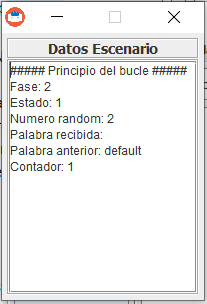
\includegraphics[height=6cm]{img/ventanaescenario}
	\caption{Ventana de escenario, para visualizar las variables de control durante la ejecución del hilo excluyente Escenario.}
	\label{figura:ventanaescenario}
\end{figure}

%%%%%%%%%%%%%%%%%%%%%%%%%%%%%%%%%%%%%%%%%%%%%%%%%%%%%%%%%%%%%%%%%%%%%%%%%%%%%%%
%                                 CONCLUSIONS                                 %
%%%%%%%%%%%%%%%%%%%%%%%%%%%%%%%%%%%%%%%%%%%%%%%%%%%%%%%%%%%%%%%%%%%%%%%%%%%%%%%

\chapter{Conclusiones}

\section{Posibles mejoras} 

Para futuras líneas de evolución de este proyecto, se pueden incorporar ciertas mejoras que pueden hacer de la aplicación entera un ente más flexible. \\

Principalmente, se asume que hoy en día la máquina virtual sobre Google Compute Engine está siempre activa. Pero a nivel de coste económico esto es bastante malo, pues los cobros en la aplicación se hacen por tiempo de uso, no por intensidad de uso. Por lo tanto, Google Compute Engine dispone de una API mediante la cual se puede activar y detener las máquinas virtuales que se deseen, así como crear nuevas o borrarlas también. Para ello es muy necesario tener buenas medidas de seguridad, pues al final las máquinas virtuales son unidades de cómputo, muy cotizadas, y cualquier desliz puede derivar en un ataque. \\

Otra mejora que facilitaría muchísimo todo el proceso es suprimir la aplicación Java en favor de una aplicación web que haga las mismas funciones pero accediendo desde el navegador. Así, se ahorra el tener que disponer del ejecutable y se convierte en una aplicación muy portable. Gracias a Google App Engine, esto es una posibilidad muy factible, pues facilita mucho las cosas para poder tener páginas web estáticas que se comunica con otros productos de Google Cloud. \\

Para solucionar la pérdida de mensajes MQTT porque un elemento se encuentra apagado y no los recibe, se puede subir el nivel de QoS, o \textit{Quality of Service}. Existen tres niveles posibles, siendo 0 el más bajo y 2 el más alto. Por defecto se encuentra a 0, que es así como se encuentra en este proyecto, y sigue la política \textit{fire and forget}, o lo que es lo mismo, envía y olvida. En el nivel 1 de QoS, cuando se recibe un mensaje, se espera un ACK, o mensaje de reconocimiento que acredita que se ha recibido el mensaje. Finalmente en el nivel 2 de QoS, se publica un mensaje, lo recibe el suscriptor, se envía un acuse de recibo que recibe el publicador, el publicador responde con que ha recibido el acuse de recibo y el suscriptor envía otro acuse de recibo. Así está explicado según HiveMQ \cite{QoS}, pero que aplica a MQTT en general. \\

Para hacer la aplicación más extensa a más robots se puede implementar en el simulador que haya más de un hilo, de forma que haya más de un simulador de diabetes para más de un robot conectado al sistema. Mediante identificaciones de ID y una buena gestión de los datos de cada uno, es asumible que puede realizarse esta mejora. \\

Finalmente si se decide prescindir de componentes de terceros como son las aplicaciones de Google, que al final suponen un coste económico, se puede adquirir un sistema empotrado, alquilar un dominio y montar allí mismo el servicio. Si bien es cierto que por ahora la aplicación tiene un coste conocido, si se decide abrir a más componentes como es más robots y más simuladores, el coste computacional sería desconocido. Entonces se perdería el beneficio de tener máquinas virtuales escalables en función de la demanda como lo hace Google Compute Engine y habría que implementarlo en el sistema empotrado mediante otra herramienta.

\section{Conclusiones}

El estado del arte en los desarrollos tiende a derivar los procesos de cómputo pesados a máquinas externas con grandes capacidades para conseguir tiempos de ejecución cada vez más competitivos. Mediante técnicas como la llevada a cabo en este proyecto es como se logra conseguir un mejor rendimiento. \\

La tecnología HTTP y la arquitectura REST, hoy en día cuasi predominantes, junto con mecanismos de comunicación asíncrona como es MQTT han permitido que este proyecto se lleve a cabo y se pueda optimizar muchísimo el código que había antes, reduciendo la cantidad de hilos y las operaciones complejas. \\

Además de los objetivos principales, que básicamente han sido reducir la carga computacional del proyecto, se ha querido optimizar el código y su implementación, es decir, corregir pequeños fallos y modernizar de acuerdo a los estándares actuales aspectos de compilación de código.

%%%%%%%%%%%%%%%%%%%%%%%%%%%%%%%%%%%%%%%%%%%%%%%%%%%%%%%%%%%%%%%%%%%%%%%%%%%%%%%
%                                BIBLIOGRAFIA                                 %
%%%%%%%%%%%%%%%%%%%%%%%%%%%%%%%%%%%%%%%%%%%%%%%%%%%%%%%%%%%%%%%%%%%%%%%%%%%%%%%

\begin{thebibliography}{10}

%%%%%%%%%%%%%%%%%%%%%%%%%%%%%%%%%%%%%%%%%%%%%%%%%%%%%%%%%%%%%%%%%%%%%%%%%%%%%%%
% MODEL D'URL                                                                 %
%%%%%%%%%%%%%%%%%%%%%%%%%%%%%%%%%%%%%%%%%%%%%%%%%%%%%%%%%%%%%%%%%%%%%%%%%%%%%%%
\bibitem{NAOWiki}
   Breve explicación de qué es el robot NAO. \\
   \newblock Consultado en: \\ 
   \url{https://es.wikipedia.org/wiki/Nao_(robot)}
   
\bibitem{NAOdatasheet}
	Características técnicas del Robot NAO. \\
	\newblock Consultado en: \\
   	\url{https://static1.squarespace.com/static/52e733d8e4b062fc0c603ea8/t/53a13620e4b0d80b1acadb20/1403074080427/nao_datashee3555555555t.pdf}

\bibitem{TFMAnterior}
	Desarrollo de un sistema de monitorización y control de un robot simulador de diabetes. Autor: Antonio Bengochea Carrasco. \\
	\newblock Consultado en: \\
	\url{https://riunet.upv.es/bitstream/handle/10251/94065/BENGOCHEA\%20-\%20Desarrollo\%20de\%20un\%20sistema\%20de\%20monitorizaci\%C3\%B3n\%20y\%20control\%20de\%20un\%20robot\%20simulador\%20de\%20diabetes.pdf?sequence=3}
	
\bibitem{ComparativaCloud}
	Cuadro comparativo con las empresas de Cloud Computing \\
	\newblock Consultado en: \\
	\url{https://recursos.apser.es/hubfs/Infograf\%C3\%ADas/APS-Cuadro-comparativo-grandes-cloud.pdf}
	
\bibitem{MQTT}
	Información sobre MQTT \\
	\newblock Consultado en: \\
	\url{http://mqtt.org/}
	
\bibitem{MQTTISO}
	ISO sobre MQTT v3.1.1 \\
	\newblock Consultado en: \\
	\url{https://www.iso.org/standard/69466.html}
	
\bibitem{MQTTComparison}
	Comparación de las implementaciones de MQTT \\
	\newblock Consultado en: \\
	\url{https://en.wikipedia.org/wiki/Comparison_of_MQTT_implementations}

\bibitem{PrincipiosHTTP}
	Principios de HTTP \\
	\newblock Consultado en: \\
	\url{https://es.wikipedia.org/wiki/Protocolo_de_transferencia_de_hipertexto}
	
\bibitem{WSGIGevent}
	WSGI de Gevent \\
	\newblock Consultado en: \\
	\url{http://www.gevent.org/}
	
\bibitem{PrincipiosREST}
	Principios de servicios RESTful \\
	\newblock Consultado en: \\
	\url{https://www.ibm.com/developerworks/ssa/library/ws-restful/index.html}
	
\bibitem{Flask}
	¿Por qué es Flask una buena elección para web? \\
	\newblock Consultado en: \\
	\url{https://www.fullstackpython.com/flask.html}
	
\bibitem{FlaskRESTful}
	Manual de la extensión de Flask para REST \\
	\newblock Consultado en: \\
	\url{https://flask-restful.readthedocs.io/en/latest/}
	
\bibitem{Alglib}
	Página principal de Alglib \\
	\newblock Consultado en: \\
	\url{http://www.alglib.net/}
	
\bibitem{Scipy}
	Página principal de la librería SciPy\\
	\newblock Consultado en: \\
	\url{https://www.scipy.org/}
	
\bibitem{C++Desaconsejado}
	Advertencia del uso de C++ para programar NAO\\
	\newblock Consultado en: \\
	\url{http://doc.aldebaran.com/2-1/getting_started/index.html}
	
\bibitem{ProgrammingLanguages}	
	Los lenguajes de programación posibles para NAO\\
	\newblock Consultado en: \\
	\url{http://doc.aldebaran.com/2-1/dev/programming_index.html}
	
\bibitem{QoS}
	Niveles de QoS, o Quality of Service en MQTT\\
	\newblock Consultado en: \\
	\url{https://www.hivemq.com/blog/mqtt-essentials-part-6-mqtt-quality-of-service-levels/}
	

\end{thebibliography}
\cleardoublepage

%%%%%%%%%%%%%%%%%%%%%%%%%%%%%%%%%%%%%%%%%%%%%%%%%%%%%%%%%%%%%%%%%%%%%%%%%%%%%%%
%                           APÈNDIXS  (Si n'hi ha!)                           %
%%%%%%%%%%%%%%%%%%%%%%%%%%%%%%%%%%%%%%%%%%%%%%%%%%%%%%%%%%%%%%%%%%%%%%%%%%%%%%%

\APPENDIX

%%%%%%%%%%%%%%%%%%%%%%%%%%%%%%%%%%%%%%%%%%%%%%%%%%%%%%%%%%%%%%%%%%%%%%%%%%%%%%%
%                         LA CONFIGURACIO DEL SISTEMA                         %
%%%%%%%%%%%%%%%%%%%%%%%%%%%%%%%%%%%%%%%%%%%%%%%%%%%%%%%%%%%%%%%%%%%%%%%%%%%%%%%

%\chapter{Configuració del sistema}

%????? ????????????? ????????????? ????????????? ????????????? ?????????????

%\section{Fase d'inicialització}

%????? ????????????? ????????????? ????????????? ????????????? ?????????????

%\section{Identificació de dispositius}

%????? ????????????? ????????????? ????????????? ????????????? ?????????????

%%%%%%%%%%%%%%%%%%%%%%%%%%%%%%%%%%%%%%%%%%%%%%%%%%%%%%%%%%%%%%%%%%%%%%%%%%%%%%%
%                               ALTRES  APÈNDIXS                              %
%%%%%%%%%%%%%%%%%%%%%%%%%%%%%%%%%%%%%%%%%%%%%%%%%%%%%%%%%%%%%%%%%%%%%%%%%%%%%%%



%%%%%%%%%%%%%%%%%%%%%%%%%%%%%%%%%%%%%%%%%%%%%%%%%%%%%%%%%%%%%%%%%%%%%%%%%%%%%%%
%                              FI DEL DOCUMENT                                %
%%%%%%%%%%%%%%%%%%%%%%%%%%%%%%%%%%%%%%%%%%%%%%%%%%%%%%%%%%%%%%%%%%%%%%%%%%%%%%%

\end{document}
